\documentclass[letterpaper,10pt,twoside]{article}

% Uncomment to include only certain sections in the output.
% \includeonly{programs/BT_ComputerScience, programs/BT_Cybersecruity}
% \includeonly{Overview, programs/AppliedComp_Business,programs/AppliedComp_Cybersecurity,AppliedComp_GraphicArts,programs/BS_Cybersecurity,plans/BS_CS-SuggestedClassSchedule, plans/BS_Cyber-SuggestedClassSchedule}
% \usepackage{excludeonly}
% \excludeonly{cover_page}

\usepackage[letterpaper, margin=0.5in, top=1in, bottom=1.25in]{geometry}
\usepackage[table]{xcolor}
\usepackage{tabularx}
\usepackage{enumitem,amssymb}
\usepackage{titlesec}
\usepackage[most]{tcolorbox}
\usepackage{graphicx}
\usepackage{fancyhdr}
\usepackage{multirow} % used only in CurriculumOfferings.tex
\usepackage{pdfpages} % for adding a PDF to this document (e.g., the cover sheet)

\usepackage[bookmarks]{hyperref}
\hypersetup{
	bookmarksnumbered=false,
	colorlinks=true,
	linkcolor=csublue,
	filecolor=csublue,
	menucolor=black,
	urlcolor=csublue,
	citecolor=csublue,
	pdftitle={Computer Science Majors Info Packet},
	pdfauthor={Sean T. Hayes, Chair},
	%pdfpagemode=FullScreen,
	pdfstartview={FitH},
}
\def\DefaultOptionsofCheckBox{print,bordercolor=black}
\def\DefaultOptionsofText{print,bordercolor=black}
\def\DefaultOptionsofText{print,bordercolor=black}

\definecolor{csublue}{HTML}{002855}
\definecolor{csugold}{HTML}{A89968}

\renewcommand{\rmdefault}{ppl} % palatino
%\renewcommand{\sfdefault}{phv}
\renewcommand{\rmdefault}{ptm}
%\renewcommand{\ttdefault}{pcr}

\graphicspath{ {./images/} }

%Set Header Style

\let\oldheadrule\headrule% Copy \headrule into \oldheadrule
\let\oldfootrule\footrule% Copy \headrule into \oldheadrule
\fancypagestyle{catalog}[fancy]{%
	\renewcommand{\headrulewidth}{1pt}
	\renewcommand{\headrule}{\color{csugold}\oldheadrule}% Add color to \headrule
	\setlength\headheight{52.5pt} %% just to make warning go away. Adjust the value after looking into the warning.
	\setlength\headsep{1em}
	\setlength\footskip{16.0pt}
	\renewcommand{\footrulewidth}{1pt}
	\renewcommand{\footrule}{{\color{csugold}\oldfootrule}\color{black}}
	%\lhead{
\includegraphics[trim={0.29in 0.35in 0 0.35in},clip,height=0.667in]{csu_logo_black}}
	\lhead{
\includegraphics[height=0.667in]{csu_logo_blue_gold}}
	\chead{\color{csublue}\large\textsc{Department of Computer Science}}
	\rhead{\color{csublue}2022--2023 Catalog}

	\cfoot{Integrating Faith in Learning, Leading, and Serving\\
	\footnotesize{{\scshape 9200 University Boulevard} \textbullet \ {\scshape PO Box 118087} \textbullet \ {\scshape Charleston, SC 29423-8087}\\
	{\scshape \href{https://charlestonsouthern.edu}{CharlestonSouthern.edu}} \textbullet \ {\scshape Phone 843-863-7369} \textbullet \ {\scshape \href{mailto:shayes@csuniv.edu?body=Dear\%20Dr.\%20Hayes,}{SHayes@csuniv.edu}}}}

	\fancyfoot[LO]{\vspace{1em}\thepage}
	\fancyfoot[RE]{\vspace{1em}\thepage}
}


\fancypagestyle{plain}{%
	\fancyhf{}% clear all header and footer fields
	\fancyfoot[C]{} % except the center
	\fancyfoot[LO]{\vspace{1em}\thepage}
	\fancyfoot[RE]{\vspace{1em}\thepage}
	\renewcommand{\headrulewidth}{0pt}%
	\renewcommand{\footrulewidth}{0pt}%
}


\newtcolorbox{reqgroup}[2][]{enhanced,colback=white,
	colframe=black,fonttitle=\bfseries,
	coltitle=black,colbacktitle=white,%enhanced,
	%attach boxed title to top center={yshift=-2mm},
	adjusted title=center,halign title=center,
	boxrule=1pt,%
	fonttitle=\bfseries\large\itshape,
	titlerule=0.5pt,
	titlerule style=csugold,
	toptitle=1pt,%
	bottomtitle=0mm,%
	top=1pt, bottom=1pt,
	middle=1pt,
	segmentation style={solid,draw=csugold},
	breakable,
	title={#2},#1
}


% Section formatting and spacing
\titleformat{\section} % command
	[display] % shape
	{\bfseries\Large\scshape} % format
	{} % label
	{0.5ex} % sep
	{
	    %\rule{\textwidth}{1pt}
	    %\vspace{1ex}
	    \centering
	} % before-code
	[
		%\hfill\vline\hfill
	] % after-code

\titleformat{\subsection} % command
	[display] % shape
	{\bfseries\large\itshape} % format
	{} % label
	{0.5ex} % sep
	{
	    %\rule{\textwidth}{1pt}
	    %\vspace{1ex}
	    \centering
	} % before-code
	[
		%\hfill\vline\hfill
	] % after-code

\titleformat{\subsubsection} % command
	[display] % shape
	{\bfseries} % format
	{} % label
	{0px} % sep
	{
	    %\rule{\textwidth}{1pt}
	    %\vspace{1ex}
	} % before-code
	[
		%\hfill\vline\hfill
	] % after-code

\titlespacing*{\section}{0pt}{0ex plus 0.2ex minus .2ex}{0.25ex plus .2ex}
\titlespacing*{\subsection}{0pt}{0ex plus 0.2ex minus .2ex}{0.25ex plus .2ex}
\titlespacing{\subsubsection}{0pt}{0ex plus 0.2ex minus .2ex}{0.25ex plus .2ex}


% Create a new checklist environment
\usepackage{pifont} % for checkmark
\newlist{checklist}{itemize}{2}
%%% Uncommnet the following two lines to use a box instead of a pdf form for the boxes.
%\setlist[checklist]{label=$\square$,topsep=0.5ex, itemsep=0.25ex, parsep=0ex}

% Use a form check box for an editable pdf
\newcounter{checkNum}% Count each checkbox so we can give them unique form-field names.
\setlist[checklist]{
	label=\stepcounter{checkNum}\setlength{\fboxsep}{1pt}\fbox{\CheckBox[width=0.6em,height=0.6em,name=box\thecheckNum,borderwidth=0bp]{\ignorespaces}},
	topsep=0.5ex, itemsep=0.25ex, parsep=0ex%
}
\newcommand{\cmark}{\ding{51}}%
\newcommand{\done}{\rlap{$\square$}{\raisebox{2pt}{\large\hspace{1pt}\cmark}}%
\hspace{-2.5pt}}

% reduce spacing between items in lists
\usepackage{enumitem}
\setlist[enumerate]{topsep=0.5ex, itemsep=0ex, parsep=0ex}
\setlist[itemize]{topsep=0.5ex, itemsep=0ex, parsep=0ex}
\setlist[description]{topsep=0.5ex, itemsep=0ex, parsep=0ex}

% Add colon after label in description lists
\renewcommand{\descriptionlabel}[1]{%
  \hspace\labelsep \upshape\bfseries #1:%
}

\newcommand{\blankReq}[0] {
	\item (\rule[-1pt]{1em}{0.5pt}) \rule[-1pt]{0.7\linewidth}{0.5pt}%
	%\item (\ChoiceMenu[combo,name=hours\thecheckNum,default=3,width=0.5em]{\mbox{}}{1,2,3,4}) \TextField[name=elective\thecheckNum,borderstyle=U,borderwidth=0.5pt,bordercolor=black,width=0.7\linewidth,height=0.9em,value=major elective]{}
}

% Rotate column in tabular to have virtical text.
\newcommand*\rotCol{\rotatebox{90}}

\setlength{\parindent}{0pt}
\setlength{\parskip}{0em}

% Reduce hypenation
\hyphenpenalty=2000

% Reduce widow/orphan lines?
\widowpenalty10000
\clubpenalty10000

\begin{document}
\pagestyle{catalog}

\phantomsection\addcontentsline{toc}{section}{Introduction to Programs}%
\section*{Want to change the world with a job you love?\\
Get a computer science degree.}
Almost half of employers have open positions for computer science graduates, according to the National Association of Colleges and Employers (NACE). Nationally, average starting salaries top the list at \$75,900! Consistently in the top 5 for job satisfaction, computer science graduates are changing the world with their skills as software developers, cybersecurity analysts, web developers, project managers, and many other roles.


\subsection{Computer Majors at Charleston Southern University}
\begin{description}

	\item[Bachelor of Science (BS) Degree in Computer Science] This challenging track of studies emphasizes the computer languages and mathematical skills necessary to enter technical job markets. Jobs in these areas are typically high-paying. Our graduates are employed by the CIA, FBI, NASA, Pentagon, Naval Information Warfare Center (NIWC), Bank of America, Blackbaud, Blue Cross Blue Shield, Bosch, Disney, Intel, Texas Instruments, Microsoft, and many others.
	\item[Bachelor of Science (BS) Degree in Cybersecurity] The degree combines coursework in computer science, network security, criminal justice, and mathematics. It is targeted towards students wishing to enter the fields of network security or information analysis.
	% \begin{minipage}[][][t]{0.69\linewidth}
	% 	\vspace{3pt}
		\item[Bachelor of Arts (BA) Degree in Applied Computing] This program is a highly flexible and challenging major for computer-related professions in business, the visual and musical arts, religious service, public service, health care, etc. Choose between concentrations in business, graphic arts, or cybersecurity.
		\item[Bachelor of Technology (BT) Degrees in Computer Science or Cybersecurity] This online degree is a special program for individuals with approved Associate Degrees. Such individuals typically transfer their Associate degrees intact with almost no loss of credits so that they can complete custom-fit four-year degrees in about two years.\vspace{0.5em}
	% \end{minipage}
	% \begin{minipage}[][][t]{0.3\linewidth}%
	% 	\hfill
	% 	% Flip the image horizontally
	% 	\scalebox{-1}[1]{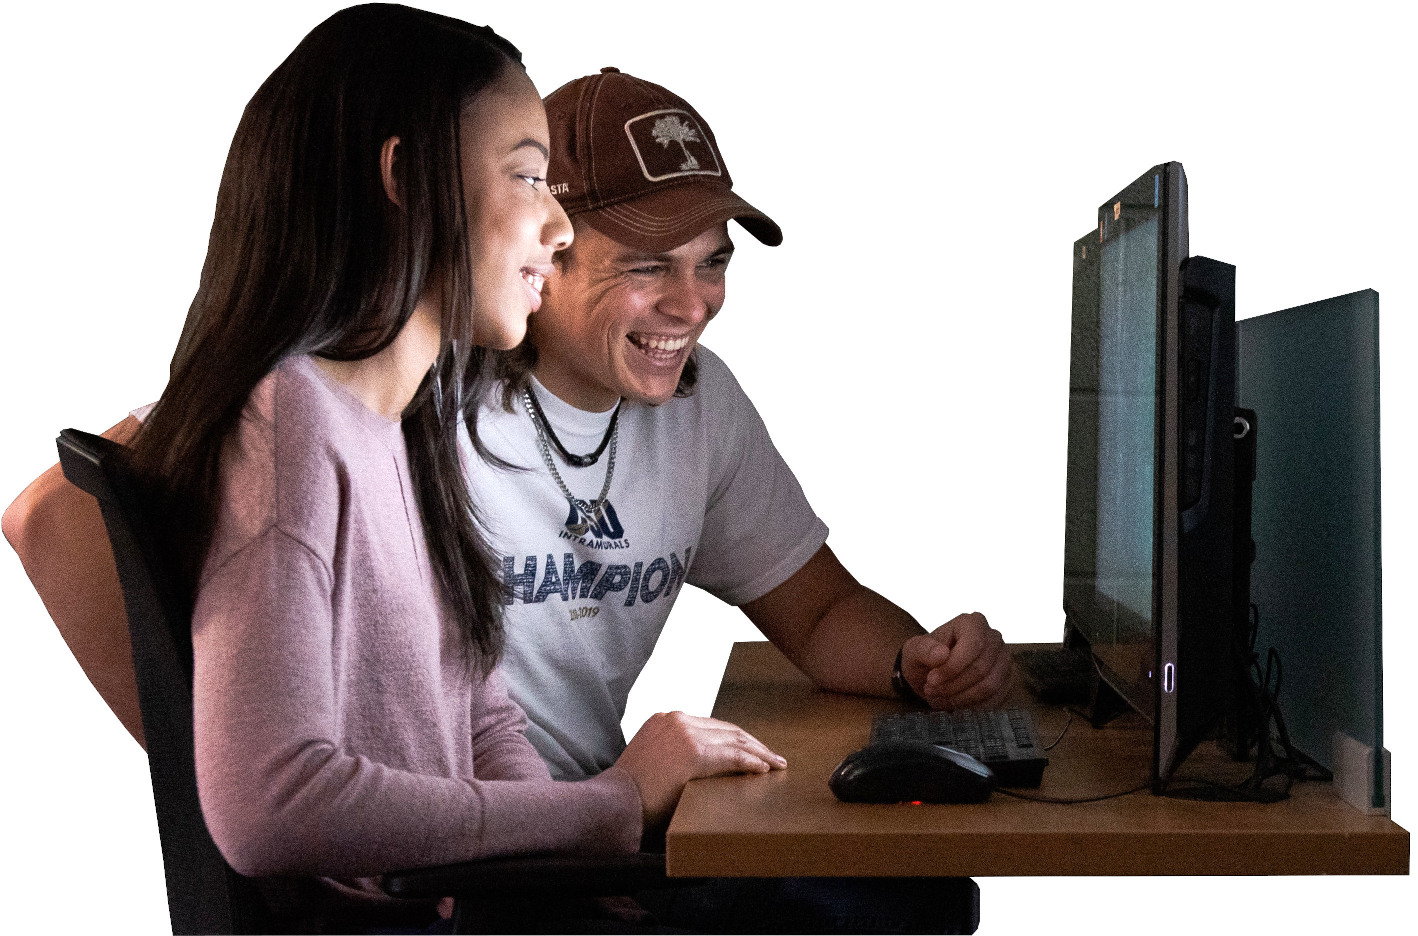
\includegraphics[width=0.95\textwidth]{SmilingTeamwork}}%
	% \end{minipage}
\end{description}

\subsection{Faculty}
\begin{description}[leftmargin=0px]
	\item[Dr. Sean Hayes] Ph.D. Computer Science, Vanderbilt University: Award-winning researcher in mobile user-interface design.
	\item[Dr. Yu-Ju (Joseph) Lin] Ph.D. Electrical \& Computer Engineering, University of Florida: Networking researcher and author.
	\item[Dr. Valerie Sessions] Ph.D. Computer Science \& Engineering, USC: Information Quality researcher, award-winning author.
	\item[Dr. Songhui Yue] Ph.D. Computer Science, University of Alabama
	\item[Prof. Julie Henderson] M.S. Computer Science, Clemson University: IBM patent holder, GIAC Certified Forensic Examiner.
	\item[Prof. Mike O’Neill] M.S. Health Physics, Georgia Institute of Technology: Database and network admin with a security focus.
	\item[Prof. Fred Worthy] M.A.T. Mathematics, Colorado State University:  From NASA. Worked on the first lunar landing.
\end{description}

\subsection{Our Unique Environment}
\begin{description}
	\item[Mission] Our mission is to incubate technically excellent, highly ethical, can-do computer professionals who will learn, lead, and serve from a Biblical worldview. To this end, we focus on the unchanging fundamentals of computer science and emphasize Christian character and ethical behavior.
	\item[Over-the-Shoulder Teaching] Involved students learn best. Consequently, most courses are taught in the lab with each student fully engaged with the computer while the subject is being taught. The faculty typically “coach” over the shoulder as opposed to delivering only standard lectures. This teaching method gives our graduates an “edge” in the workplace.
	\item[Small Class Size] Computer classes do not exceed 24 students per class and are usually smaller.
	\item[Emphasis on Teamwork] Teamwork is critical to success in the information technology workplace. For this reason, our courses stress teamwork in-class assignments. Students learn to apply team dynamics to accomplish complex tasks.
	\item[Focus on the Real World] Our goal is to produce well-rounded graduates who can succeed in the real world.  To this end, each student must complete a year-long, senior project under the direction of a mentor and defend it orally. During the project, each student must demonstrate independent research, self-learn the skills needed, then design and complete the project to the customer’s satisfaction.  Each must also pass a comprehensive exit exam.
	\item[Graduate Program] Students can earn a master’s degree in CS with only one additional year of school.
	\item[Web Site] \href{https://charlestonsouthern.edu/computer-science}{charlestonsouthern.edu/computer-science}
\end{description}
\phantomsection\addcontentsline{toc}{section}{Introduction to Programs}%
\section*{Want to change the world with a job you love?\\
Get a computer science degree.}
Almost half of employers have open positions for computer science graduates, according to the National Association of Colleges and Employers (NACE). Nationally, average starting salaries top the list at \$75,900! Consistently in the top 5 for job satisfaction, computer science graduates are changing the world with their skills as software developers, cybersecurity analysts, web developers, project managers, and many other roles.


\subsection{Computer Majors at Charleston Southern University}
\begin{description}

	\item[Bachelor of Science (BS) Degree in Computer Science] This challenging track of studies emphasizes the computer languages and mathematical skills necessary to enter technical job markets. Jobs in these areas are typically high-paying. Our graduates are employed by the CIA, FBI, NASA, Pentagon, Naval Information Warfare Center (NIWC), Bank of America, Blackbaud, Blue Cross Blue Shield, Bosch, Disney, Intel, Texas Instruments, Microsoft, and many others.
	\item[Bachelor of Science (BS) Degree in Cybersecurity] The degree combines coursework in computer science, network security, criminal justice, and mathematics. It is targeted towards students wishing to enter the fields of network security or information analysis.
	% \begin{minipage}[][][t]{0.69\linewidth}
	% 	\vspace{3pt}
		\item[Bachelor of Arts (BA) Degree in Applied Computing] This program is a highly flexible and challenging major for computer-related professions in business, the visual and musical arts, religious service, public service, health care, etc. Choose between concentrations in business, graphic arts, or cybersecurity.
		\item[Bachelor of Technology (BT) Degrees in Computer Science or Cybersecurity] This online degree is a special program for individuals with approved Associate Degrees. Such individuals typically transfer their Associate degrees intact with almost no loss of credits so that they can complete custom-fit four-year degrees in about two years.\vspace{0.5em}
	% \end{minipage}
	% \begin{minipage}[][][t]{0.3\linewidth}%
	% 	\hfill
	% 	% Flip the image horizontally
	% 	\scalebox{-1}[1]{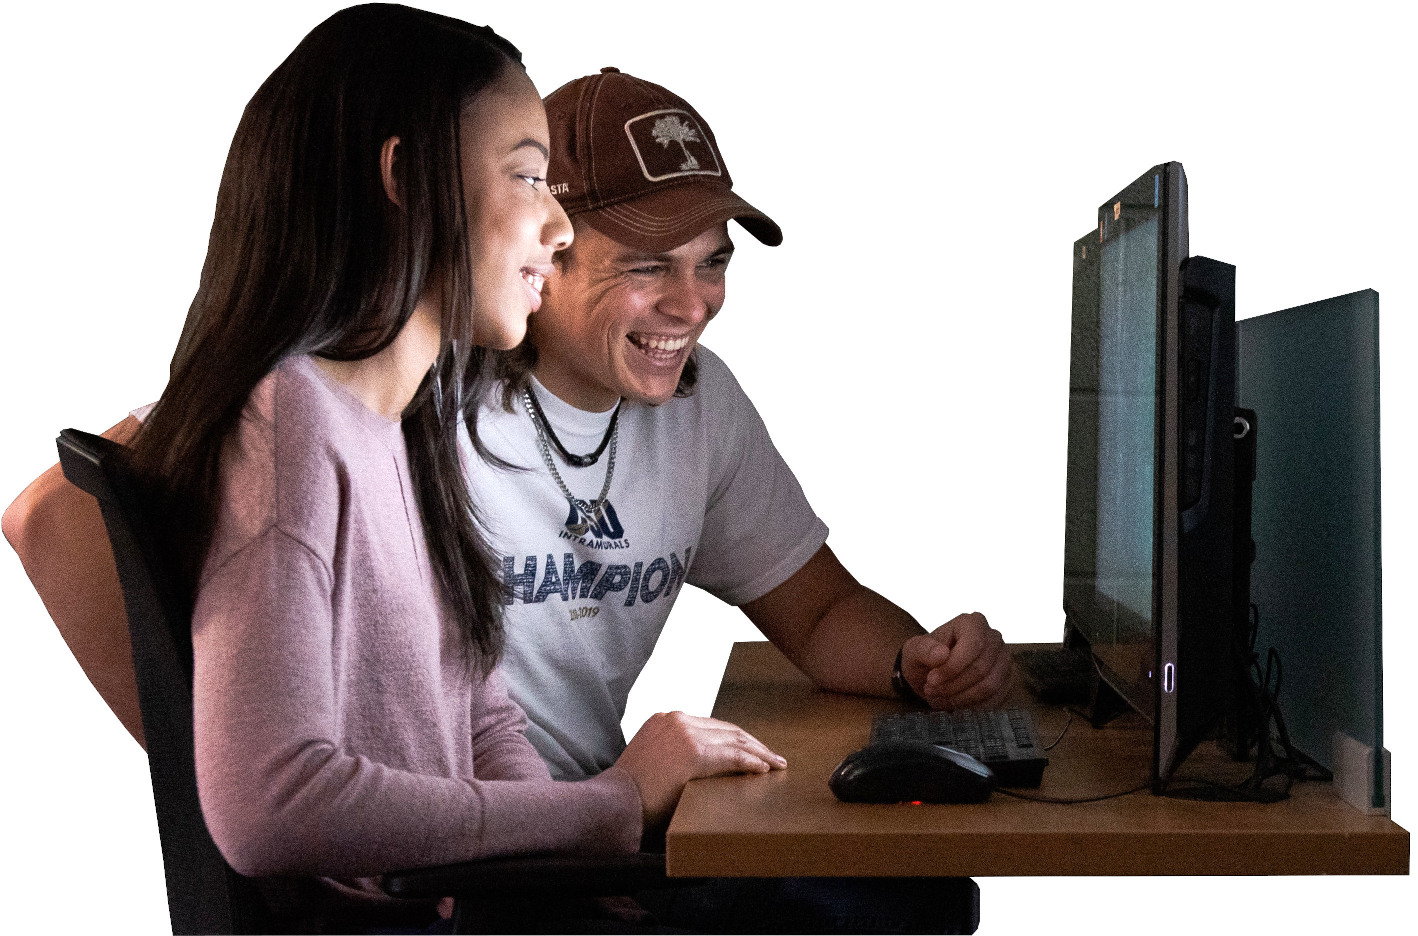
\includegraphics[width=0.95\textwidth]{SmilingTeamwork}}%
	% \end{minipage}
\end{description}

\subsection{Faculty}
\begin{description}[leftmargin=0px]
	\item[Dr. Sean Hayes] Ph.D. Computer Science, Vanderbilt University: Award-winning researcher in mobile user-interface design.
	\item[Dr. Yu-Ju (Joseph) Lin] Ph.D. Electrical \& Computer Engineering, University of Florida: Networking researcher and author.
	\item[Dr. Valerie Sessions] Ph.D. Computer Science \& Engineering, USC: Information Quality researcher, award-winning author.
	\item[Dr. Songhui Yue] Ph.D. Computer Science, University of Alabama
	\item[Prof. Julie Henderson] M.S. Computer Science, Clemson University: IBM patent holder, GIAC Certified Forensic Examiner.
	\item[Prof. Mike O’Neill] M.S. Health Physics, Georgia Institute of Technology: Database and network admin with a security focus.
	\item[Prof. Fred Worthy] M.A.T. Mathematics, Colorado State University:  From NASA. Worked on the first lunar landing.
\end{description}

\subsection{Our Unique Environment}
\begin{description}
	\item[Mission] Our mission is to incubate technically excellent, highly ethical, can-do computer professionals who will learn, lead, and serve from a Biblical worldview. To this end, we focus on the unchanging fundamentals of computer science and emphasize Christian character and ethical behavior.
	\item[Over-the-Shoulder Teaching] Involved students learn best. Consequently, most courses are taught in the lab with each student fully engaged with the computer while the subject is being taught. The faculty typically “coach” over the shoulder as opposed to delivering only standard lectures. This teaching method gives our graduates an “edge” in the workplace.
	\item[Small Class Size] Computer classes do not exceed 24 students per class and are usually smaller.
	\item[Emphasis on Teamwork] Teamwork is critical to success in the information technology workplace. For this reason, our courses stress teamwork in-class assignments. Students learn to apply team dynamics to accomplish complex tasks.
	\item[Focus on the Real World] Our goal is to produce well-rounded graduates who can succeed in the real world.  To this end, each student must complete a year-long, senior project under the direction of a mentor and defend it orally. During the project, each student must demonstrate independent research, self-learn the skills needed, then design and complete the project to the customer’s satisfaction.  Each must also pass a comprehensive exit exam.
	\item[Graduate Program] Students can earn a master’s degree in CS with only one additional year of school.
	\item[Web Site] \href{https://charlestonsouthern.edu/computer-science}{charlestonsouthern.edu/computer-science}
\end{description}

\begin{Form}[NeedAppearances=true]
\phantomsection\addcontentsline{toc}{section}{BS in Computer Science}%
\section*{Bachelor of Science: Computer Science}

\begin{reqgroup}{Liberal Arts Core Requirements (49 hours)}
%\subsection*{}
\begin{checklist}
\begin{minipage}[t]{0.5\linewidth}
	\item (3) ENGL 111 or 180 Composition and Rhetoric 1 *
	\item (3) ENGL 112 Composition and Rhetoric 2 *
	\item (3) ENGL 202, 203, or 204 Literature
	\item (3) COMM 110 Public Speaking
	\item (3) Any 3-hour foreign language course
	\item (4) \textbf{CSCI 235  Procedural Programming} *
	\item (3) CHST 111  Survey of the Old Testament
	\item (3) CHST 112  Survey of the New Testament
	\item (3) HIST 111, 112, or 113 Western Civ.
\end{minipage}
\begin{minipage}[t]{0.5\linewidth}
	\item (3)	Another History, POLI 201, or CHST 140
	\item (3)	ART 202 Art Appr, or MUSI 171 or 371, or THEA 218 or 311
	\item (3)	BUSI 203, CRIM 210, ECON 211, ECON 212, HEAL 201, POLI 101, PSYC 110, or SOCI 101, 203, or 205
	\item (4)	\textbf{MATH 221 Calculus I} *
	\item (4)	CHEM 121, BIOL 161, PHYS 201 or PHYS 203
	\item (4)	Lab Science\\Limited one lab science course per category of Biology, Chemistry,
Geology, or Physics.
\end{minipage}
\end{checklist}
\end{reqgroup}

%\vspace{1em}

\begin{reqgroup}{Computer Science/Mathematics Requirements (60--63 hours)}
\begin{checklist}
\begin{minipage}[t]{0.5\linewidth}
	\item (3) MATH 213 Probability and Statistics\\or MATH 346 (3) \& MATH 347 (3)
	\item (4) MATH 222 Calculus II
	\item (4) MATH 321 Calculus III\\or MATH 326 Linear Algebra
	\item (3) MATH 330 Discrete Mathematics

	\item (4) CSCI 301 Survey of Scripting Languages
	\item (4) CSCI 315 Data Structure Analysis
	\item (4) CSCI 325 Object-Oriented Programming
	\item (4) CSCI 330 Computer Architecture
	\item (4) CSCI 332 Applied Networking
	\item (4) CSCI 415 Algorithms
	\item (4) CSCI 419 Database Management


\end{minipage}
\begin{minipage}[t]{0.5\linewidth}
	\item (4) CSCI 431 Operating Systems
	\item (0) CSCI 490 Computer Science Exit Exam
	\item (3) CSCI 495 Systems Analysis and Software Design
	\item (0) CSCI 496 Senior Portfolio Review
	\item (1) CSCI 497 Senior Project Design
	\item (1) CSCI 498 Senior Project Construction
	\item (1) CSCI 499 Senior Project Implementation/Defense

	\item (8) Eight Elective CSCI hours from:
	\item \hspace{1em}\begin{minipage}[t]{\dimexpr\linewidth-1em\relax}CSCI 322 Multimedia (4); 334 User-Interface (4); 360 Mobile App Dev.; 409 Artfcl Intl (4); 432 Mobile/Wireless Ntwk (4); 433 Ntwk Security(4); 434 Human-Comp. Inter. (4); 435 Adv. Ntwk (4); 442 Data Mining (4); 450 Graphics (4); 452 Net. Pen., Test., \& Ethical Hacking (4); or other approved CSCI elective at 300/400 level\end{minipage}


\end{minipage}
\end{checklist}
\end{reqgroup}

\begin{reqgroup}{General Electives (11 hours)}
Any 11 hours can be taken; however, the following are suggested or may be required as prerequisites.
\begin{checklist}
\begin{minipage}[t]{\linewidth}
	\item (1)	GNED 101	First-Year Seminar
	\item (3--4)	CSCI 217	Practical Programming and Problem Solving or CSCI 215	Programming in Alice
	\item (3--4) Math 110 or 111 College Algebra
	\item (4) MATH 130 Precalculus
\end{minipage}
\end{checklist}
\end{reqgroup}

Notes:%
\begin{enumerate}\footnotesize
	\item This major is
		\href{https://www.abet.org/accreditation/what-is-accreditation/why-abet-accreditation-matters/}{accreddited by the Computing Accreditation Commission of ABET}.
	\item This major does not require a minor.
	\item * Indicates courses that must be completed within the first four major terms (Fall and Spring).
	\item If prerequisites are needed for the cognate requirements, summer courses may be required for four-years completion.
	\item Residency requirement: 36 of the last 46 hours must be earned while attending CSU. Of these, at least 12 must be 300--400 level courses.
	\item Students may request one official degree audit through their \href{https://portal.csuniv.edu/}{MyCSU account}, which is recommended during the next to last semester.
	\item Students are responsible for applying to graduate. See the Registrar.
	\item Full-time day students must meet chapel requirements. See the Student Development section of the catalog.
	\item In cases of conflict between this checklist and the catalog, the catalog takes precedence.
\end{enumerate}
\phantomsection\addcontentsline{toc}{section}{BS in Cybersecurity}%
\section*{Bachelor of Science: Cybersecurity}

\begin{reqgroup}{Liberal Arts Core Requirements (49 hours)}
%\subsection*{}
\begin{checklist}
\begin{minipage}[t]{0.5\linewidth}
	\item (3) ENGL 111 or 180 Composition and Rhetoric *
	\item (3) ENGL 112 Composition with Intro\@. to Literature *
	\item (3) English 202, 203, or 204 Literature
	\item (3) COMM 110 Public Speaking
	\item (3) Any 3-hour foreign language course
	\item (4) \textbf{CSCI 235  Procedural Programming} *
	\item (3) CHST 111  Survey of the Old Testament
	\item (3) CHST 112  Survey of the New Testament
	\item (3) HIST 111, 112, or 113 Western Civ.
\end{minipage}
\begin{minipage}[t]{0.5\linewidth}
	\item (3) Another History, POLI 201, or CHST 140
	\item (3) ART 202 Art Appr, or MUSI 171 or 371, or THEA 218 or 311
	\item (3) \textbf{CRIM 210 Introduction to Criminal Justice}
	\item (4) \textbf{MATH 221 Calculus I} *
	\item (4) Lab Science
	\item (4) Lab Science\\Limited one lab science course per category of Biology, Chemistry,
Geology, or Physics.
\end{minipage}
\end{checklist}
\end{reqgroup}

%\vspace{1em}

\begin{reqgroup}{Computer Science/Mathematics Requirements (52 hours)}
\begin{checklist}
\begin{minipage}[t]{0.5\linewidth}
	\item (3) MATH 213 Probability and Statistics
	\item (3) MATH 330 Discrete Mathematics
	\item (4) CSCI 301 Survey of Scripting Languages
	\item (4) CSCI 325 Object-Oriented Programming
	\item (4) CSCI 330 Computer Architecture
	\item (4) CSCI 332 Applied Networking
	\item (4) CSCI 352 Cyber Defense
	\item (3) CSCI 405 Principles of Cybersecurity
	\item (4) CSCI 433 Network Security
	\item (4) CSCI 452 Network Penetration Testing and\\Ethical Hacking
\end{minipage}
\begin{minipage}[t]{0.5\linewidth}
	\item (0) CSCI 491 Cybersecurity Exit Exam $^4$
	\item (0) CSCI 496 Senior Portfolio Review
	\item (1) CSCI 497 Senior Project Design
	\item (1) CSCI 498 Senior Project Construction
	\item (1) CSCI 499 Senior Project Implementation/Defense
	\item (12) Elective CSCI hours from: CSCI 315 Data Structures;
	\item \hspace{1em} CSCI 419 Database Management; CSCI 409 Mobile App
	\item \hspace{1em} Development; CSCI 434 Data Mining, CSCI 316
	\item[] \hspace{1em} Competitive Security, or other 300/400 CSCI course


\end{minipage}
\end{checklist}
\end{reqgroup}

\begin{reqgroup}{Criminal Justice Requirements (9 hours)}
\begin{checklist}
\begin{minipage}[t]{0.5\linewidth}
	\item (3) CRIM 212 - Techniques of Criminal Investigations
\end{minipage}
\begin{minipage}[t]{0.5\linewidth}
	\item (3) Criminal Justice electives at the 200 level or higher
	\item (3) Criminal Justice electives at the 200 level or higher
\end{minipage}
\end{checklist}
Recommended courses include CRIM 232 Current Issues and Trends in Criminal Justice,
CRIM 455 Homeland Security, and CRIM 312 Advanced Criminal Justice Techniques
\end{reqgroup}

\begin{reqgroup}{General Electives (10 hours)}
Any 10 hours can be taken; however, the following are suggested or may be required as prerequisites.
\begin{checklist}
\begin{minipage}[t]{\linewidth}
	\item (1)	GNED 101	First-Year Seminar
	\item (3--4)	CSCI 217	Practical Programming and Problem Solving or CSCI 215	Programming in Alice
	\item (3--4) Math 110 or 111 College Algebra
	\item (4) MATH 130 Precalculus
	\item (4) MATH 222 Calculus II \em{Recommended for students considering employment in the federal government.}
\end{minipage}
\end{checklist}
\end{reqgroup}

Notes:%
\begin{enumerate}\footnotesize
	\item This major is
		\href{https://www.abet.org/accreditation/what-is-accreditation/why-abet-accreditation-matters/}{accreddited by the Computing Accreditation Commission of ABET} and does not require a minor.
	\item * Indicates courses that must be completed within the first four major terms (Fall and Spring).
	\item If prerequisites are needed for the cognate requirements, summer courses may be required for four-years completion.
	\item The exit exam is the \href{https://www.comptia.org/certifications/security}{CompTIA Security+ Certification} exam.
	\item Residency requirement: 36 of the last 46 hours must be earned while attending CSU. Of these, at least 12 must be 300--400 level courses.
	\item Students may request one official degree audit through their \href{https://portal.csuniv.edu/}{MyCSU account}, which is recommended during the next-to-last semester.
	\item Students are responsible for applying to graduate. See the Registrar.
	\item Full-time day students must meet chapel requirements. See the Student Development section of the catalog.
	\item In cases of conflict between this checklist and the catalog, the catalog takes precedence.
\end{enumerate}
\phantomsection\addcontentsline{toc}{section}{BA in Applied Computing with a Business Concentration}%
\section*{Bachelor of Arts: Applied Computing with a Business Concentration}

\begin{reqgroup}{Liberal Arts Core Requirements (48--49 hours)}
%\subsection*{}
\begin{checklist}
\begin{minipage}[t]{0.5\linewidth}
	\item (3) ENGL 111 or 180 Composition and Rhetoric
	\item (3) ENGL 112 Composition with Intro\@. to Literature
	\item (3) ENGL 202, 203, or 204 Literature
	\item (3) COMM 110 Public Speaking
	\item (3) Any 3-hour foreign language course
	\item (4) \textbf{CSCI 235  Procedural Programming}
	\item (3) CHST 111  Survey of the Old Testament
	\item (3) CHST 112  Survey of the New Testament
	\item (3) HIST 111, 112, or 113 Western Civ.
\end{minipage}
\begin{minipage}[t]{0.5\linewidth}
	\item (3)	Another History, POLI 201, or CHST 140
	\item (3)	ART 202 Art Appr, or MUSI 171 or 371, or THEA 218 or 311
	\item (3)	\textbf{ECON 211 or ECEC 203 Microeconomics}
	\item (3--4)	\textbf{Math 110 or 111 College Algebra}
	\item (4)	Lab Science
	\item (4)	Lab Science\\Limited one lab science course per category of Biology, Chemistry,
Geology, or Physics.
\end{minipage}
\end{checklist}
\end{reqgroup}

%\vspace{1em}

\begin{reqgroup}{Core Major Studies (26 hours)}
\begin{checklist}
\begin{minipage}{0.5\linewidth}
	\item (4) CSCI 301	Survey of Scripting Languages
	\item (4) CSCI 315	Data Structure Analysis
	\item (4) CSCI 325	Object-Oriented Programming
	\item (4) CSCI 332	Applied Networking
\end{minipage}
\begin{minipage}{0.5\linewidth}
	\item (4) CSCI 419	Database Management
	\item (0) CSCI 492	Applied Computing Exit Exam
	\item (4) CSCI 495	Systems Analysis and Software Design
	\item (3) MATH 213	Probability and Statistics
	\end{minipage}
\end{checklist}
\end{reqgroup}

\begin{reqgroup}{Business Concentration (40 hours)}
\begin{center}%
(This concentration can be completed completely online.)\vspace{-0.5em}%
\end{center}%
\begin{checklist}
\begin{minipage}[t]{0.5\linewidth}
	\item (3) MATH 209	Calculus for Business
	\item (3) CSCI/CRIM 405	Principles of Cybersecurity
	\item (0) CSCI 496	Senior Portfolio Review
	\item (1) CSCI 497	Senior Project Design
	\item (1) CSCI 498	Senior Project Construction
	\item (1) CSCI 499	Senior Project Implementation/Defense
	\item (4) CSCI elective at 300/400 level
\end{minipage}
\begin{minipage}[t]{0.5\linewidth}
	\item (3) ECON 211 / ECEC 203 Microeconomics
	\item (3) ECON 212 / ECEC 204 Macroeconomics
	\item (3) ACCT 210 / ECBA 202	Accounting I or Accounting Principles for Managers
	\item (3) MGMT 310 / ECBA 301	Management
	\item (3) MRKT 310 / ECBA 308	Marketing
\end{minipage}
\end{checklist}

\tcblower

An additional 15 hours may come from any courses at the 300 level or above from the following categories: \\ACCT (including ACCT 211), BUSI (except 314), CSCI, ECBA, FINA, MATH, MGMT or MRKT.
\begin{checklist}
\begin{minipage}[t]{0.5\linewidth}
	\blankReq
	\blankReq
	\blankReq
\end{minipage}
\begin{minipage}[t]{0.5\linewidth}
	\blankReq
	\blankReq
\end{minipage}
\end{checklist}
\end{reqgroup}

\begin{reqgroup}{General Electives (6 hours)}
Any 6 hours can be taken; however, the following are suggested or may be required as prerequisites.
\begin{checklist}
\begin{minipage}[t]{\linewidth}
	\item (1)	GNED 101	First-Year Seminar
	\item (3--4)	CSCI 217	Practical Programming and Problem Solving or CSCI 215	Programming in Alice%\\
	% \begin{minipage}[t]{0.5\linewidth}
		\blankReq
	% \end{minipage}
	% \begin{minipage}[t]{0.5\linewidth}
	% 	\blankReq
	% \end{minipage}
\end{minipage}
\end{checklist}
\end{reqgroup}

Notes:%
\begin{enumerate}\footnotesize
	\item This major does not require a minor.
	\item To complete in four years, students must begin cognate requirements in the freshman year. If prerequisites are needed before beginning the cognate requirements, summer courses may be required to move into the proper scheduling cycle for four-years completion.
	\item Residency requirement: 36 of the last 46 hours must be earned while attending CSU. Of these, at least 12 must be 300--400 level courses.
	\item Students may request one official degree audit through their MyCSU account, which is recommended during the next to last semester.
	\item Students are responsible for applying to graduate. See the Registrar.
	\item Full-time day students must meet chapel requirements. See the Student Development section of the catalog.
	\item In cases of conflict between this checklist and the catalog, the catalog takes precedence.
\end{enumerate}
\phantomsection\addcontentsline{toc}{section}{BA in Applied Computing with a Cybersecurity Concentration}%
\section*{Bachelor of Arts: Applied Computing\\with a Cybersecurity Concentration}

\begin{reqgroup}{Liberal Arts Core Requirements (48--49 hours)}
%\subsection*{}
\begin{checklist}
\begin{minipage}[t]{0.5\linewidth}
	\item (3) ENGL 111 or 180 Composition and Rhetoric
	\item (3) ENGL 112 Composition with Intro\@. to Literature
	\item (3) ENGL 202, 203, or 204 Literature
	\item (3) COMM 110 Public Speaking
	\item (3) Any 3-hour foreign language course
	\item (4) \textbf{CSCI 235  Procedural Programming}
	\item (3) CHST 111  Survey of the Old Testament
	\item (3) CHST 112  Survey of the New Testament
	\item (3) HIST 111, 112, or 113 Western Civ.
\end{minipage}
\begin{minipage}[t]{0.5\linewidth}
	\item (3)	Another History, POLI 201, or CHST 140
	\item (3)	ART 202 Art Appr, or MUSI 171 or 371, or THEA 218 or 311
	\item (3)	\textbf{CRIM 210 Introduction to Criminal Justice}
	\item (3--4)	\textbf{Math 110 or 111 College Algebra}
	\item (4)	Lab Science
	\item (4)	Lab Science\\Limited one lab science course per category of Biology, Chemistry,
Geology, or Physics.
\end{minipage}
\end{checklist}
\end{reqgroup}

%\vspace{1em}

\begin{reqgroup}{Core Major Studies (26 hours)}
\begin{checklist}
\begin{minipage}{0.5\linewidth}
	\item (4) CSCI 301	Survey of Scripting Languages
	\item (4) CSCI 315	Data Structure Analysis
	\item (4) CSCI 325	Object-Oriented Programming
	\item (4) CSCI 332	Applied Networking
\end{minipage}
\begin{minipage}{0.5\linewidth}
	\item (4) CSCI 419	Database Management
	\item (0) CSCI 491	Cybersecurity Exit Exam 
	\item (4) CSCI 495	Systems Analysis and Software Design
	\item (3) MATH 213	Probability and Statistics
	\end{minipage}
\end{checklist}
\end{reqgroup}

\begin{reqgroup}{Cybersecurity Concentration (40 hours)}
\begin{center}%
(This concentration can be completed completely online.)\vspace{-0.5em}%
\end{center}%
\begin{checklist}
\begin{minipage}[t]{0.5\linewidth}
	\item (4) CSCI 352 Cyber Defense
	\item (3) CSCI 405 Principles of Cybersecurity
	\item (4) CSCI 433 Network Security
	\item (0) CSCI 496 Senior Portfolio Review
\end{minipage}
\begin{minipage}[t]{0.5\linewidth}
	\item (1) CSCI 497 Senior Project Design
	\item (1) CSCI 498 Senior Project Construction
	\item (1) CSCI 499 Senior Project Implementation/Defense
	\item (3) CRIM 227 Critical Thinking/Writing in Criminal Justice
\end{minipage}
\end{checklist}

\tcblower

An additional 23 hours may come from any courses at the 300 level or above from the following categories:\\CRIM (including 212, 232, and 255), CSCI, and MATH.
\begin{checklist}
\begin{minipage}[t]{0.5\linewidth}
	\blankReq
	\blankReq
	\blankReq
	\blankReq
\end{minipage}
\begin{minipage}[t]{0.5\linewidth}
	\blankReq
	\blankReq
	\blankReq
	\blankReq
\end{minipage}
\end{checklist}
\end{reqgroup}

\begin{reqgroup}{General Electives (6 hours)}
Any 6 hours can be taken; however, the following are suggested or may be required as prerequisites.
\begin{checklist}
\begin{minipage}[t]{\linewidth}
	\item (1)	GNED 101	First-Year Seminar
	\item (3--4)	CSCI 217	Practical Programming and Problem Solving or CSCI 215	Programming in Alice%\\
	% \begin{minipage}[t]{0.5\linewidth}
		\blankReq{}
	% \end{minipage}
	% \begin{minipage}[t]{0.5\linewidth}
	% 	\blankReq
	% \end{minipage}
\end{minipage}
\end{checklist}
\end{reqgroup}

Notes:%
\begin{enumerate}\footnotesize
	\item This major does not require a minor.
	\item For completion is four years, students must begin cognate requirements in the freshman year. If prerequisites are needed for cognate requirements, summer courses may be required to move into the proper scheduling cycle.
	\item Residency requirement: 36 of the last 46 hours must be earned while attending CSU. Of these, at least 12 must be 300--400 level courses.
	\item Students may request one official degree audit through their MyCSU account, which is recommended during the next to last semester.
	\item Students are responsible for applying to graduate. See the Registrar.
	\item Full-time day students must meet chapel requirements. See the Student Development section of the catalog.
	\item In cases of conflict between this checklist and the catalog, the catalog takes precedence.
\end{enumerate}

\phantomsection\addcontentsline{toc}{section}{BA in Applied Computing with a Graphic Arts Concentration}%
\section*{Bachelor of Arts: Applied Computing\\with a Graphic Arts Concentration}

\begin{reqgroup}{Liberal Arts Core Requirements (48--49 hours)}
\begin{checklist}
\begin{minipage}[t]{0.5\linewidth}
	\item (3) English 111
	\item (3) English 112
	\item (3) English 202, 203 or 204
	\item (3) COMM 110 Public Speaking
	\item (3) Any 3-hour foreign language course
	\item (4) \textbf{CSCI 235  Procedural Programming}
	\item (3) CHST 111  Survey of the Old Testament
	\item (3) CHST 112  Survey of the New Testament
	\item (3) History 111, 112 or 113 Western Civ.
\end{minipage}
\begin{minipage}[t]{0.5\linewidth}
	\item (3)	Another History, POLI 201, or CHIST 140
	\item (3)	\textbf{ART 202 Art Appreciation}
	\item (3)	BUSI 203, CRIM 210, ECON 211, ECON 212, HEAL 201, POLI 101, PSYC 110, or SOCI 101, 203, or 205
	\item (3--4)	\textbf{Math 110 or 111 College Algebra}
	\item (4)	 Lab Science
	\item (4)	 Lab Science\\Limited one lab science course per category of Biology, Chemistry,
Geology, or Physics.
\end{minipage}
\end{checklist}
\end{reqgroup}

\begin{reqgroup}{Core Major Studies (26 hours)}
\begin{checklist}
\begin{minipage}{0.5\linewidth}
	\item (4) CSCI 301	Survey of Scripting Languages
	\item (4) CSCI 315	Data Structure Analysis
	\item (4) CSCI 325	Object-Oriented Programming
	\item (4) CSCI 332	Applied Networking
\end{minipage}
\begin{minipage}{0.5\linewidth}
	\item (4) CSCI 419	Database Management
	\item (4) CSCI 490	Computer Science Exit Exam
	\item (4) CSCI 490	Computer Science Exit Exam
	\item (4) CSCI 495	Systems Analysis and Software Design
	\item (4) MATH 213	Probability and Statistics
	\end{minipage}
\end{checklist}
\end{reqgroup}

\begin{reqgroup}{Graphic Arts Concentration  (40 hours)}
\begin{center}%
(This concentration requires on-campus courses.)\vspace{-0.5em}%
\end{center}%
\begin{checklist}
\begin{minipage}[t]{0.5\linewidth}
	\item (3) ART 215 Beginning Design
	\item (3) ART 216 Visual Communications
	\item (3) ART 221 Digital Image Editing
	%\item (3) ART 318 Advertising Design
	\item (3) ART 341 Web Design I
	\item (3) ART 418 Business of Design
	\item (3) ART 441 Web Design II
\end{minipage}
\begin{minipage}[t]{0.5\linewidth}
	\item (0) CSCI 496 Senior Portfolio Review
	\item (1) CSCI 497 Senior Project Design
	\item (1) CSCI 498 Senior Project Construction
	\item (1) CSCI 499 Senior Project Implementation/Defense
	\item (4) CSCI elective at 300/400 level
	\item (3) CSCI elective at 300/400 level
\end{minipage}
\end{checklist}

\tcblower

An additional 12 hours may come from any courses at the 300 level or above from the following categories: ART or CSCI
\begin{checklist}
\begin{minipage}[t]{0.5\linewidth}
	\blankReq
	\blankReq
\end{minipage}
\begin{minipage}[t]{0.5\linewidth}
	\blankReq
	\blankReq
\end{minipage}
\end{checklist}
\end{reqgroup}

\begin{reqgroup}{General Electives (11 hours)}
Any 11 hours can be taken; however, the following are suggested or may be required as prerequisites.
\begin{checklist}
\begin{minipage}[t]{\linewidth}
	\item (1)	GNED 101	First-Year Seminar
	\item (3--4)	CSCI 217	Practical Programming and Problem Solving or CSCI 215	Programming in Alice\\
	\begin{minipage}[t]{0.5\linewidth}
		\blankReq
	\end{minipage}
	\begin{minipage}[t]{0.5\linewidth}
		\blankReq
	\end{minipage}
\end{minipage}
\end{checklist}
\end{reqgroup}

Notes:%
\begin{enumerate}\footnotesize
	\item This major does not require a minor.
	\item To complete in four years, students must begin cognate requirements in the freshman year. If prerequisites are needed before beginning the cognate requirements, summer courses may be required to move into the proper scheduling cycle for four-years completion.
	\item Graduates must meet residency requirements. 36 of the last 46 hours must be earned while attending CSU. Of these, at least 12 must be 300-400 level courses.
	\item Students may request one official degree audit through their MyCSU account, which is recommended during the next to last semester.
	\item Students are responsible for applying to graduate. See the Registrar.
	\item Full-time day students must meet chapel requirements. See the Student Development section of the catalog.
	\item In cases of conflict between this checklist and the catalog, the catalog takes precedence.
\end{enumerate}

\phantomsection\addcontentsline{toc}{section}{BT in Computer Science}%
\section*{Bachelor of Technology: Computer Science}
\begin{reqgroup}{General Information}
\begin{itemize}\small

	\item The Bachelor of Technology (BT) is a baccalaureate program for individuals with approved associate degrees. You may transfer your approved degree intact up to 89 credit hours and earn an accredited 4-year degree in about two years of full-time work.

	\item Your BT degree is individually tailored based on courses diverse courses transferred in, your goals, course availability, academic viability, etc. Consequently, the BT degree is flexible to your situation and focused on you.

	\item In addition to transferred credit, you must complete: all outstanding core courses, the cognate, and any elective courses to total at least 125 credit hours (including associate degree credit).

	\item To apply for the BT, contact CSU Admissions at:
		\href{https://apply.charlestonsouthern.edu/}{apply.charlestonsouthern.edu} (Undergraduate Admissions), or at (843) 863-7050 or (800) 947-7474.\\
		Have your official transcripts sent to the Office of Admissions (address at the bottom of the page below). Indicate BT on the application.

	\item For more information, ask at: \href{https://www.charlestonsouthern.edu/contact-us/}{charlestonsouthern.edu/contact-us/} .


	\item When the evaluation is done, the Registrar will assign you to an advisor. Contact your advisor to plan your BT degree.
\end{itemize}
\end{reqgroup}

\begin{reqgroup}{Liberal Arts Core Requirements (48--50 hours)}
\begin{checklist}
\begin{minipage}[t]{0.5\linewidth}
	\item (3) ENGL 111 or 180 Composition and Rhetoric 1
	\item (3) ENGL 112 Composition and Rhetoric 2
	\item (3) ENGL 202, 203, or 204 Literature
	\item (3) COMM 110 Public Speaking
	\item (3) Any 3-hour foreign language course
	\item (3--4) Any CSCI course
	\item (3) CHST 111  Survey of the Old Testament
	\item (3) CHST 112  Survey of the New Testament
	\item (3) HIST 111, 112, or 113 Western Civ.
\end{minipage}
\begin{minipage}[t]{0.5\linewidth}
	\item (3) Another History, POLI 201, or CHST 140
	\item (3) ART 202 Art Appr, or MUSI 171 or 371, or THEA 218 or 311
	\item (3) BUSI 203, CRIM 210, ECON 211, ECON 212, HEAL 201, POLI 101, PSYC 110, or SOCI 101, 203, or 205
	\item (3--4) \textbf{MATH 110 College Algebra} (or higher)
	\item (4) Lab Science
	\item (4) Lab Science\\Limited one lab science course per category of Biology, Chemistry,
Geology, or Physics.
\end{minipage}
\end{checklist}
\end{reqgroup}

%\vspace{1em}

\begin{reqgroup}{Computer Science/Mathematics Cognate (18 hours)}%
\begin{center}%
	(At least 15 of these hours must be 300 level or above.)\vspace{-0.5em}%
\end{center}%
\begin{checklist}%
\begin{minipage}[t]{0.5\linewidth}%
	\item (3) MATH 213 Probability and Statistics
	\item (3) CSCI 215 Programming in Alice
	\item (4) CSCI 217 Practical Programming and Prob. Solving
	\item (4) CSCI 235	Procedural Programming *
	\item (4) CSCI 301 Survey of Scripting Languages *
	\item (2) CSCI 306 Competitive Programming
	\item (4) CSCI 325 Object-Oriented Programming *
\end{minipage}%
\begin{minipage}[t]{0.5\linewidth}
	\item (4) CSCI 334 User-Interface Programming
	\item (4) CSCI 332 Applied Networking
	\item (4) CSCI 352 Cyber Defense
	\item (3) CSCI 405 Principles of Cybersecurity
	\item (4) CSCI 419 Database Management *
	\item (3) CSCI 495 Systems Analysis and Software Design
	\item (0) CSCI 496 Senior Portfolio Review (\em{required}) *
\end{minipage}
\end{checklist}
\end{reqgroup}

\begin{reqgroup}{General Electives}
All non-cognate courses used for the required 125-hour graduation minimum, prerequisites, or other requirements.
\end{reqgroup}

Notes:%
\begin{enumerate}\footnotesize
	\item No more than 89 hours from sources other than baccalaureate degree-granting institutions may be used toward the BT degree. However, accepted, non-associate degree credit from baccalaureate institutions might be used.
	\item CSCI 496 Senior Portfolio is required for graduation. See CSCI 496 in catalog for detail.
	\item If prerequisites are needed for the cognate requirements, summer courses may be required for four-years completion.
	\item Residency requirements: 36 of the last 46 hours must be earned while attending CSU. Of these, \textbf{at least 15} must be 300-400 level courses.
	\item Students may request one official degree audit through their \href{https://portal.csuniv.edu/}{MyCSU account}. Recommending during the next to last semester.
	\item BT candidates who miss two consecutive major semesters must revise the degree plan for any new requirements.
	\item Students are responsible to complete an Application for Graduation. See Registrar.
	\item Full-time day students must meet chapel requirements. See the Student Development section of the catalog.
	\item In cases of conflict between this checklist and the catalog, the catalog takes precedence.
\end{enumerate}
\phantomsection\addcontentsline{toc}{section}{BT in Cybersecurity}%
\section*{Bachelor of Technology: Cybersecurity}

\begin{reqgroup}{General Information}
\begin{itemize}\small

	\item The Bachelor of Technology (BT) is a baccalaureate program for individuals with approved associate degrees. You may transfer your approved degree intact up to 89 credit hours and earn an accredited 4-year degree in about two years of full-time work.

	\item Your BT degree is individually tailored based on courses diverse courses transferred in, your goals, course availability, academic viability, etc. Consequently, the BT degree is flexible to your situation and focused on you.

	\item In addition to transferred credit, you must complete: all outstanding core courses, the cognate, and any elective courses to total at least 125 credit hours (including associate degree credit).

	\item To apply for the BT, contact CSU Admissions at:
		\href{https://apply.charlestonsouthern.edu/}{apply.charlestonsouthern.edu} (Undergraduate Admissions), or at (843) 863-7050 or (800) 947-7474.\\
		Have your official transcripts sent to the Office of Admissions (address at the bottom of the page below). Indicate BT on the application.

	\item For more information, ask at: \href{https://www.charlestonsouthern.edu/contact-us/}{charlestonsouthern.edu/contact-us/} .


	\item When the evaluation is done, the Registrar will assign you to an advisor. Contact your advisor to plan your BT degree.
\end{itemize}
\end{reqgroup}

\begin{reqgroup}{Liberal Arts Core Requirements (48--50 hours)}
\begin{checklist}
\begin{minipage}[t]{0.5\linewidth}
	\item (3) English 111
	\item (3) English 112
	\item (3) English 202, 203 or 204
	\item (3) COMM 110 Public Speaking
	\item (3) Any 3-hour foreign language course
	\item (3--4) Any CSCI course
	\item (3) CHST 111  Survey of the Old Testament
	\item (3) CHST 112  Survey of the New Testament
	\item (3) History 111, 112 or 113 Western Civ.
\end{minipage}
\begin{minipage}[t]{0.5\linewidth}
	\item (3)	Another History, POLI 201, or CHIST 140
	\item (3)	ART 202 Art Appr, or MUSI 171 or 371, or THEA 218 or 311
	\item (3)	BUSI 203, CRIM 210, ECON 211, ECON 212, HEAL 201, POLI 101, PSYC 110, or SOCI 101, 203, or 205
	\item (3--4)	\textbf{MATH 110 College Algebra} (or higher)
	\item (4)	Lab Science
	\item (4)	Lab Science\\Limited one lab science course per category of Biology, Chemistry,
Geology, or Physics.
\end{minipage}
\end{checklist}
\end{reqgroup}

%\vspace{1em}

\begin{reqgroup}{Cybersecurity Cognate (19 hours)}%
\begin{checklist}%
\begin{minipage}[t]{0.5\linewidth}%
	\item (4) CSCI 235 Procedural Programming
	\item (4) CSCI 301 Survey of Scripting Languages\\
		or CSCI 352 Cyber Defense
	\item (4) CSCI 332 Applied Networking
\end{minipage}%
\begin{minipage}[t]{0.5\linewidth}
	\item (3) CSCI 405 Principles of Cybersecurity
	\item (4) CSCI 433 Network Security
	\item (0) CSCI 496 Senior Portfolio Review
\end{minipage}
\end{checklist}
\end{reqgroup}

\begin{reqgroup}{General Electives}
All non-cognate courses used for the required 125-hour graduation minimum, prerequisites, or other requirements.
\end{reqgroup}

Notes:%
\begin{enumerate}\footnotesize
	\item No more than 89 hours from sources other than baccalaureate degree-granting institutions may be used toward the BT degree. However, accepted, non-associate degree credit from baccalaureate institutions might be used.
	\item CSCI 496 Senior Portfolio is required for graduation. See CSCI 496 in catalog for detail.
	\item If prerequisites are needed for the cognate requirements, summer courses may be required for four-years completion.
	\item Graduates must meet residency requirements. 36 of the last 46 hours must be earned while attending CSU. Of these, \textbf{at least 15} must be 300-400 level courses.
	\item Students may request one official degree audit through their \href{https://portal.csuniv.edu/}{MyCSU account}. Recommending during the next to last semester.
	\item BT candidates who miss two consecutive major semesters must revise the degree plan for any new requirements.
	\item Students are responsible to complete an Application for Graduation. See Registrar.
	\item Full-time day students must meet chapel requirements. See the Student Development section of the catalog.
	\item In cases of conflict between this checklist and the catalog, the catalog takes precedence.
\end{enumerate}
\phantomsection\addcontentsline{toc}{section}{Minor in Applied Computing}%
\section*{Minor in Applied Computing}

\begin{reqgroup}{Core Courses Required for All Tracks (7--8 hours)}
\begin{checklist}
\begin{minipage}[t]{0.5\linewidth}
	\item (3--4) CSCI 215 Programming in Alice or CSCI 217 Practical Programming and Problem Solving
	\item (4) CSCI 235	Procedural Programming
\end{minipage}
\begin{minipage}[t]{0.5\linewidth}
\end{minipage}
\end{checklist}
\end{reqgroup}

\vspace{1em}
\subsection*{Choose one of the following tracks}

\begin{reqgroup}{Computer Programming Track (11--12 hours)}
\begin{checklist}
	\item (4) CSCI 332 Applied Networking
	\item (4) CSCI 325 Object-Oriented Programming
	\item (3--4) Any 300/400 level CSCI course that does not duplicate a course in the major.
\end{checklist}
\end{reqgroup}

\begin{reqgroup}{Cybersecurity Track (11 hours)}
\begin{checklist}
	\item (3) CSCI/CRIM 405 Principles of Cybersecurity
	\item (4) CSCI 301 Survey of Scripting Languages
	\item (4) CSCI 352 Cyber Defense
\end{checklist}
\end{reqgroup}

\begin{reqgroup}{Information Systems Track (11--12 hours)}
\begin{checklist}
	\item (4) CSCI 419 Database Management
	\item (4) CSCI 495 Systems Analysis and Software Design
	\item (3--4) Any 300/400 level CSCI course that does not duplicate a course in the major.
\end{checklist}
\end{reqgroup}

\begin{reqgroup}{Web Development Track (14 hours)}
\begin{checklist}
	\item (3) ART 216 Visual Communications
	\item (3) ART 221 Digital Image Editing
	\item (4) CSCI 332 Applied Networking
	\item (4) CSCI 334 User-Interface Programming
\end{checklist}
\end{reqgroup}

Notes:%
\begin{enumerate}\footnotesize
	\item Math 110 or higher is a prerequisite and satisfies the Math Liberal Arts Core.
	\item Computer courses should generally be taken in the order listed due to prerequisites.
	\item Courses used in the major cannot be duplicated in the minor.
	\item Graduates must meet residency requirements. The current catalog’s residency requirements are: 36 of the last 46 hours must be earned while attending CSU. Of these, at least 12 hrs must be 300--400 level courses in the major, and at least 6 hrs must be 300--400 level courses in the minor.
	\item In cases of conflict between this checklist and the catalog, the catalog takes precedence.
\end{enumerate}
\phantomsection\addcontentsline{toc}{section}{MS in Computer Science}%
\section*{Master of Science: Computer Science}

The Master of Science in Computer Science degree is designed to provide an advanced understanding of the technical fundamentals of computer science: architecture, database, networking, and software engineering. The non-thesis program of study is designed to enhance professional development for those currently working in the field while providing advanced skills and knowledge to those seeking employment in the field. The thesis program of study provides the basis for further advanced study in the field. Reflected in the programs of study is a commitment to the highest ethical, intellectual, and social values.

\begin{reqgroup}{MSCS Core Courses (18 hours)}
%\subsection*{}
\begin{checklist}
\begin{minipage}[t]{0.5\linewidth}
	\item (3) CSCI 515  Advanced Algorithms
	\item (3) CSCI 531  Advanced Operating Systems
	\item (3) CSCI 535  Advanced Computer Networks
\end{minipage}
\begin{minipage}[t]{0.5\linewidth}
	\item (3) CSCI 540  Software Testing and Maintenance
	\item (3) CSCI 541  Distributed Database Systems
	\item (3) CSCI 560  Advanced Computer Architecture
\end{minipage}
\end{checklist}
\end{reqgroup}

%\vspace{1em}

\begin{reqgroup}{Major Electives (12 hours from)}
\begin{center}%
(Choose any combination of the following courses. Students perusing the thesis track must take CSCI 697 \& CSCI 698.)\vspace{-0.5em}%
\end{center}%
\begin{checklist}
\begin{minipage}[t]{0.5\linewidth}
	\item (3) CSCI 534  Human-Computer Interaction
	\item (3) CSCI 542  Data Mining
	\item (3) CSCI 552  Network Penetration, Testing, \&\\Ethical Hacking
	\item (3) CSCI 555  Compiler Construction
	\item (3) CSCI 590  Applied Cryptography
\end{minipage}
\begin{minipage}[t]{0.5\linewidth}
	\item (3) CSCI 635  Advanced Topics in Network Security
	\item (3) CSCI 640  Open-Source Software Engineering
	\item (1) CSCI 650  Fieldwork
	\item (3) CSCI 697  Research I
	\item (3) CSCI 698  Research II
\end{minipage}
\end{checklist}
\end{reqgroup}

Notes:%
\begin{enumerate}\footnotesize
	\item To earn a Master of Science in Computer Science from Charleston Southern University (CSU), a student must form a graduation committee and pass either a Written Final Examination (non-thesis track) or a Thesis Review (thesis track).
	\item In cases of conflict between this checklist and the catalog, the catalog takes precedence.
\end{enumerate}
\end{Form}

\section{Curriculum Offerings by Semester}

% \begin{tabular}{c@{ = }l}
% 	\checkmark & offered every year\\%
% 	O & offered only in \emph{odd} calendar years\\%
% 	E & offered only in \emph{even} calendar years%
% \end{tabular}
\begin{center}
\setlength{\arrayrulewidth}{1pt}
\rowcolors{5}{white}{gray!20}
\begin{tabular}{ | r@{\hspace{3pt} }c@{\hspace{3pt} }l | c c c | c c c | c c c | }
	\cline{4-12}
	\multicolumn{3}{l|}{}&&&&&&&&&\\[-0.5em] % Extra row to get a little more height
	\multicolumn{3}{l|}{This is a tentative plan and is subject to change without notice.}
		& \multicolumn{3}{c|}{\large Fall} & \multicolumn{3}{c|}{\large Spring} & \multicolumn{3}{c|}{\large Summer} \\
	\multicolumn{3}{l|}{%
		\multirow{-3}{*}{
			\begin{tabular}{c@{ = }l}
				\checkmark & offered every year\\%
				O & offered only in \emph{odd} calendar years\\%
				E & offered only in \emph{even} calendar years%
			\end{tabular}}}%
		& \rotCol{Day} & \rotCol{Evening} & \rotCol{Online}
		& \rotCol{Day} & \rotCol{Evening} & \rotCol{Online}
		& \rotCol{Day} & \rotCol{Evening} & \rotCol{Online}\\
	\hline
	GNED 101 & (1) & First-Year Seminar & \checkmark & &    & & &    & & & \\
	\hline
	MATH 111 & (3) & College Algebra            & \checkmark & &    & \checkmark & & & \checkmark & & \\
	MATH 130 & (4) & Precalculus                & \checkmark & &    & \checkmark & &    & \checkmark & & \\
	MATH 209 & (3) & Calculus for Business      & & & \checkmark    & \checkmark & &    & & & \\
	MATH 213 & (3) & Probability and Statistics & \checkmark & &    & & & \checkmark   & & & \\
	MATH 221 & (4) & Calculus I                 & \checkmark & &    & \checkmark & &    & & & \\
	MATH 222 & (4) & Calculus II                & \checkmark & &    & \checkmark & &    & & & \\
	MATH 321 & (4) & Calculus III               & \checkmark & &    & \checkmark & &    & & & \\
	MATH 326 & (4) & Linear Algebra             & & &               & \checkmark & &    & & & \\
	MATH 330 & (3) & Discrete Mathematics       & \checkmark & &    & \checkmark & &    & & & \\
	\hline
	%CSCI 209 & (3) & Introduction to Computer Systems & \checkmark & &    & & &    & & & \\
	CSCI 210 & (3) & Intro. to Computer Science through Robotics &  &  & \checkmark   & \checkmark & & \checkmark   & & & \\
	CSCI 211 & (3) & Intro. to Computers for Business Applications & \checkmark & &    & \checkmark & &    & & & \\
	CSCI 215 & (3) & Programming in Alice & \checkmark & & \checkmark   & \checkmark & & \checkmark   & & & \checkmark \\
	CSCI 217 & (4) & Practical Programming and Problem Solving & \checkmark & &    & \checkmark & &    & & & \\
	CSCI 235 & (4) & Procedural Programming & \checkmark & \checkmark & \checkmark   & \checkmark & \checkmark & \checkmark   & & & \\
	CSCI 301 & (4) & Survey of Scripting Languages & & \checkmark & \checkmark    & \checkmark & & \checkmark    & & & \\
	CSCI 306 & (2) & Competitive Programming & \checkmark & &    & & &    & & & \\
	CSCI 315 & (4) & Data Structure Analysis & \checkmark & & \checkmark    & \checkmark & & \checkmark    & & & \\
	CSCI 316 & (2) & Competitive Security &  & &    & \checkmark & &    & & & \\
	CSCI 322 & (4) & Multimedia & & &    & & E &    & & & \\
	CSCI 325 & (4) & Object-Oriented Programming & \checkmark & & \checkmark    & \checkmark & & \checkmark    & & & \\
	CSCI 330 & (4) & Computer Architecture & & &    & \checkmark & & \checkmark    & & & \\
	CSCI 332 & (4) & Applied Networking & \checkmark & & \checkmark    & & \checkmark & \checkmark    & & & \\
	CSCI 334 & (4) & User-Interface Programming & & &    & & & \checkmark    & & & \\
	CSCI 352 & (4) & Cyber Defense & & &    & & \checkmark &    & & & \\
	CSCI 360 & (4) & Intro to Mobile Application Development & & &    & & &    & & & O \\
	\multicolumn{2}{|c}{CSCI 371--374} & Student-Directed Coursework in CS & \checkmark & &    & \checkmark & &    & & & \\
	CSCI 405 & (3) & Principles of Cybersecurity & & \checkmark &    & & \checkmark & \checkmark    & & & \\
	CSCI 409 & (4) & Fundamentals of Artificial Intelligence & & E &    & & &    & & & \\
	CSCI 415 & (4) & Algorithms & \checkmark & &    & & &    & & & \\
	CSCI 419 & (4) & Database Management & & & \checkmark    & & & & & & \\
	CSCI 431 & (4) & Operating Systems & \checkmark & &    & & &    & & & \\
	CSCI 432 & (4) & Mobile and Wireless Networks & & E &    & & &    & & & \\
	CSCI 433 & (4) & Network Security & & \checkmark &    & & \checkmark &    & & & \\
	CSCI 434 & (4) & Human-Computer Interaction & & & \checkmark    & & &    & & & \\
	CSCI 435 & (4) & Advanced Computer Networks & & O &    & & &    & & & \\
	CSCI 442 & (4) & Data Mining & & & O    & & &    & & & \\
	CSCI 452 & (4) & Network Penetration, Testing and Ethical Hacking & & &    & & \checkmark &    & & & \\
	CSCI 469 & (4) & Computer Science Internship & \checkmark & &    & \checkmark & &    & & & \\
	CSCI 495 & (3) & Systems Analysis and Software Design & & & \checkmark    & & &    & & & \\
	\multicolumn{2}{|c}{CSCI 496--499} & Portfolio and Senior Project & \checkmark & &    & \checkmark & &    & & & \\

	\hline
	CRIM 227 & (3) & Critical Thinking and Writing in Criminal Justice & \checkmark & &    & & & \checkmark    & & & \\
	\hline
\end{tabular}
\end{center}
\section{Curriculum Prerequisites}
\begin{center}Note: Prerequisites must be completed with a C or better.\end{center}
\setlength{\tabcolsep}{5pt}
\setlength{\arrayrulewidth}{1px}

%\begin{table}[!ht]
\begin{reqgroup}[left*=1pt,right*=1pt,bottom=0pt]{}
\centering\small
\rowcolors{0}{white}{gray!20}
\begin{tabularx}{\textwidth}{ r c l  | X }
%\hline
\multicolumn{3}{c}{\normalsize\textbf{Course}} & \multicolumn{1}{c}{\normalsize\textbf{Prerequisite(s)}}\\
\arrayrulecolor{csugold}\hline
	GNED 101 & (1) & First-Year Seminar & \\

	MATH 111 & (3) & College Algebra & MATH 099 or departmental placement \\
	MATH 130 & (4) & Precalculus & MATH 110 or 111 \\
	MATH 209 & (3) & Calculus for Business & MATH 110 or 111 \\
	MATH 213 & (3) & Probability and Statistics & MATH 110 or 111 \\
	MATH 221 & (4) & Calculus I & MATH 130 or departmental placement \\
	MATH 222 & (4) & Calculus II & MATH 221 \\
	MATH 321 & (4) & Calculus III & MATH 222 \\
	MATH 326 & (4) & Linear Algebra & MATH 222 \\
	MATH 330 & (3) & Discrete Mathematics & MATH 221  \\

	CSCI 215 & (3) & Programming in Alice &\\
	CSCI 217 & (4) & Practical Programming and Problem Solving & Corequisite: MATH 110 or higher\\
	CSCI 235 & (4) & Procedural Programming                              & CSCI 215, 217, or instructor's permission and MATH 110 or higher \\
	CSCI 301 & (4) & Survey of Scripting Languages                       & CSCI 235 \\
	CSCI 306 & (2) & Competitive Programming                             & CSCI 325 or co-requisite MATH 326 \\
	CSCI 312 & (3) & Quantitative Modeling and Computer Simulation       & MATH 110 or higher \\
	CSCI 315 & (4) & Data Structure Analysis                             & CSCI 325 \\
	CSCI 316 & (2) & Competitive Security                                & CSCI 301 \\
	%CSCI 322 & (4) & Multimedia                                          &  CSCI 332 \\
	CSCI 325 & (4) & Object-Oriented Programming                         & CSCI 325 \\
	CSCI 326 & (4) & Java Programming II                                 &  CSCI 325 \\
	CSCI 330 & (4) & Computer Architecture                               & MATH 330 and CSCI 325 \\
	CSCI 332 & (4) & Applied Networking                                  & CSCI 235 \\
	%CSCI 333 & (4) & Applied Systems                                     & CSCI 315 \\
	CSCI 334 & (4) & User-Interface Programming                          & CSCI 332 \\
	CSCI 352 & (4) & Cyber Defense                                       & CSCI 301 \\
	CSCI 360 & (4) & Intro to Mobile Application Development                         & CSCI 332 \\
	CSCI 371--374 & (1--4) & Student-Directed Coursework in Computer Science & CSCI 235, submission of proposed coursework to faculty supervisor and Department of Computer Science Chair 4 weeks prior to beginning of course, and approval of the Department of Computer Science Chair \\
	CSCI 383 & (3) & Creative Teamwork                                   & Permission of the instructor \\
	CSCI 401--403 & (1--3) & Computer Science Research                   & 16 CSCI hours and instructor permission \\
	CSCI 405 & (3) & Principles of Cybersecurity                         & CSCI 215, CSCI 217, or CSCI 235 \\
	CSCI 409 & (4) & Fundamentals of Artificial Intelligence             & CSCI 315 \\
	CSCI 415 & (4) & Algorithms                                          & CSCI 315 \\
	CSCI 419 & (4) & Database Management                         & CSCI 235 or 12 hours in BUSI \\
	CSCI 431 & (4) & Operating Systems                         & CSCI 315 and CSCI 330 \\
	CSCI 432 & (4) & Mobile and Wireless Networks                         & CSCI 332 \\
	CSCI 433 & (4) & Network Security                         & CSCI 332 with a grade of C or better \\
	CSCI 434 & (4) & Human-Computer Interaction                         & CSCI 334 and MATH 213 \\
	%CSCI 435 & (4) & Computer Networks                         & CSCI 325 and 332 \\
	CSCI 442 & (4) & Data Mining                         & CSCI 419 and MATH 213 \\
	CSCI 450 & (4) & Graphics                         & CSCI 315 and MATH 130 \\
	CSCI 452 & (4) & Network Penetration, Testing and Ethical Hacking    & CSCI 330 and CSCI 332 \\
	CSCI 469--470 & (1--4) & Computer Science Internship                  & Computer Science major, 61 semester hours, 2.75 GPA, at least one semester as a CSU student, and permission of the Department of Science Chair \\
	CSCI 490 & (0) & Computer Science Exit Exam                         &  CSIC 315 or CSCI 325 \& MATH 213 \\
	CSCI 495 & (3) & Systems Analysis and Software Design               & CSCI 325 or CSCI 419 \\
	CSCI 496 & (1) & Senior Portfolio Review                         & Instructor permission \\
	CSCI 497--499 & (1) & Senior Project                         & Instructor permission \\
\end{tabularx}
\end{reqgroup}

%\end{table}
\phantomsection\addcontentsline{toc}{section}{BS in CS Class Schedule}%
\section*{Bachelor of Science: Computer Science}
\begin{center}
Suggested Class Schedule for Computer Science and Math Courses.
% \def\svgwidth{0.9\textwidth}
% \input{./images/PrerequisiteDiagram_BS_ComputerScience.pdf_tex}

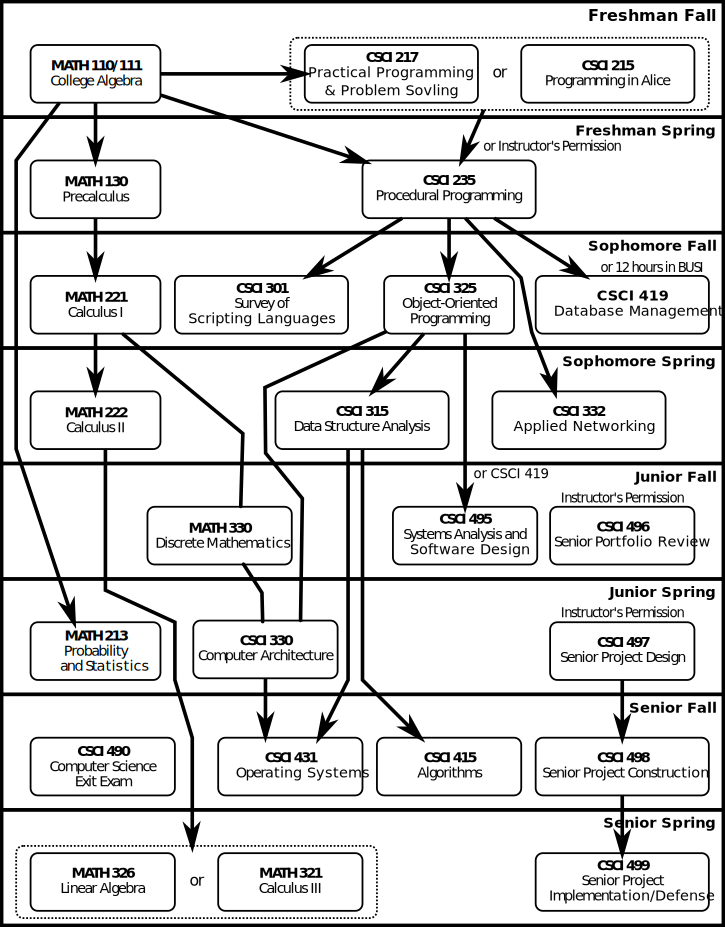
\includegraphics[width=0.86\textwidth]{images/PrerequisiteDiagram_BS_ComputerScience}
\end{center}
\phantomsection\addcontentsline{toc}{section}{BS in Cybersecurity Class Schedule}%
\section*{Bachelor of Science: Cybersecurity}
\begin{center}
Suggested Class Schedule for Computer Science, Math, and Criminal Justice Courses.
% \def\svgwidth{0.9\textwidth}
% \input{./images/PrerequisiteDiagram_BS_ComputerScience.pdf_tex}

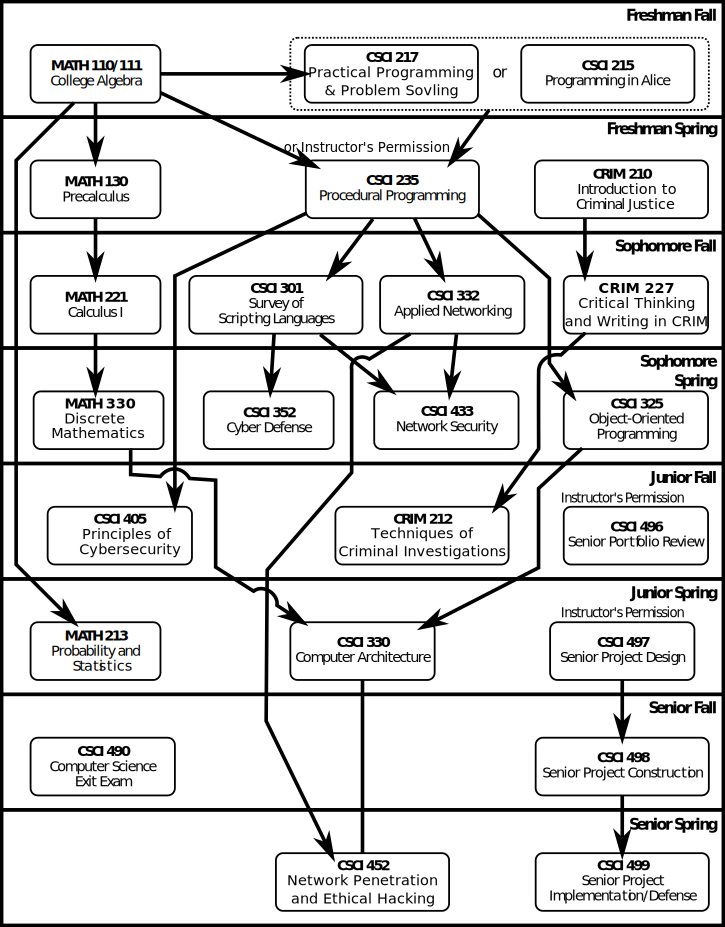
\includegraphics[width=0.86\textwidth]{images/PrerequisiteDiagram_BS_Cybersecurity}
\end{center}
\section{Course Descriptions for CSCI Programs}

\subsection{Business}
\subsubsection{ACCT 210 -- Principles of Accounting I}
(3 hours) Prerequisite: MATH 105 or higher. The preparation and use of financial statements based on Generally Accepted Accounting Principles, as applied to sole proprietorships, partnerships, and corporations. This course cannot be challenged.

\subsubsection{ACCT 211 -- Principles of Accounting II}
(3 hours) Prerequisite: ACCT 210 (grade of “C” or better). The preparation, analysis, and interpretation of accounting information in planning, controlling and managing a business organization. This course cannot be challenged.

\subsubsection{ECON 211 -- Principles of Microeconomics}
(3 hours) Prerequisites: MATH 110 (or higher) and ENGL 111. An introductory study of the parts of the economy including consumers, firms, industries, and markets. Firm pricing and resource allocation. This course cannot be challenged.

\subsubsection{ECON 212 -- Principles of Macroeconomics}
(3 hours) Prerequisites: MATH 110 (or higher) and ENGL 111. An introduction to the economy as a whole. National income, employment, prices and inflation, and output in an economic system. Problems in controlling and forecasting economic fluctuations. This course cannot be challenged.

\subsubsection{MRKT 310 -- Principles of Marketing}
(3 hours) Prerequisites: ACCT 210. Concepts involved in the planning, pricing, promotion, and distribution of goods and services. This course cannot be challenged.

\subsubsection{MGMT 310 -- Principles of Management}
(3 hours) Prerequisites: MRKT 310 (grade of “C” or better). An interdisciplinary approach to the analysis and application of psychological, social, and cultural influences on the behavior of consumers and organizational buyers. The interrelationships of marketing actions and buyer behavior are analyzed with the goal of making effective marketing decisions. This course cannot be challenged.

\subsubsection{MATH 098 -- Elementary Algebra Review}
(1 hour) Prerequisite: SAT Math below 440 or student requests/advisor suggests course for review purposes. A review of the concepts of Elementary Algebra to help prepare the student for MATH 111. This course is graded Pass or Fail. The hour earned does not count toward graduation.

\subsection{Criminal Justice}

\subsubsection{CRIM 210 -- Introduction to Criminal Justice}
(3 hours) An introduction to Criminal Justice, including philosophical background, history, constitutional limits, agencies, processes of justice, and evaluation of current criminal justice practices.

\subsubsection{CRIM 212 -- Techniques of Criminal Investigations}
(3 hours) Prerequisite: CRIM 210. A study of investigative techniques used in crime scene analysis. These include but are not limited to, examination of questioned documents, fingerprint techniques, polygraph examinations, firearms identifications ballistics, toxicology, pathology, interrogation and interviewing, and photography.

\subsubsection{CRIM 227 -- Critical Thinking and Writing in Criminal Justice}
(3 hours) Prerequisites: CRIM 210 and ENGL 111. An introductory overview of basic research methods and writing for the criminal justice student. Attention will be given to online and traditional avenues of research, as well as standard formats for case briefs and police investigative documents.

\subsubsection{CRIM 232 -- Current Issues and Trends in Criminal Justice}
(3 hours) Prerequisite: CRIM 210. This course provides an examination of the current issues and trends within the criminal justice system. The student will develop an up-to-date awareness of activities within today’s criminal justice system in the areas of police, courts, and corrections. Integration of faith from both a contemporary and biblical perspective will be intertwined in the definition of Justice.

\subsubsection{CRIM 312 -- Advanced Criminal Investigative Techniques}
(3 hours) Prerequisites: CRIM 210 and 212. This is an advanced level course for Criminal Justice majors and minors. The focus of the class will be to combine the art of investigation with the science of criminalistics.  Advances in forensics have vastly changed the criminal investigative process, and this course will integrate academic and applied approaches to advance the development of criminal investigative techniques for the undergraduate student. Laboratory fee required.

\subsubsection{CRIM 455 -- Homeland Security}
(3 hours) Prerequisites: CRIM 210 and junior/senior status. This course will define the relatively new criminal justice field of Homeland Security as well as identify and explore the definition of terrorism. The course will also visit the aspects of Counter Terrorism and Anti-Terrorism as it applies to the criminal justice discipline.


\subsection{Computer Science}

\subsubsection{CSCI 215 -- Programming in Alice}
(3 hours) An introduction to computer programming using Alice. Basic computer functionality and data representations are learned within Alice’s 3D programming environment that makes it easy to create animated stories and interactive games. The development of critical thinking skills in the area of problem-solving is a major focus. This course is not a substitute for courses requiring CSCI 209 as a prerequisite. Lecture 2 hours, laboratory 2 hours. (Laboratory fee required for on-ground classes.)

\subsubsection{CSCI 217 -- Practical Programming and Problem Solving}
(4 hours) Corequisite or Prerequisite: MATH 110 or higher. A practical introduction to computer programming in the context of personal task optimization, entertainment, and industry. Without prior programming experience, develop computational thinking skills, gain the satisfying abilities to identify a problem, create an effective solution, see the results, and share it with others. Confidently write small programs to accomplish useful goals. Programming topics may include personal finance, business tools, mathematics, games, sports, simulators, and more utilizing various programming constructs such as data types, decisions, repetition, functions, arrays, and file handling. Lecture 3 hours, laboratory 2 hours. (Laboratory fee required for on-ground classes.)

\subsubsection{CSCI 235 -- Procedural Programming}
(4 hours) Prerequisites: CSCI 215 or 217 or permission of the instructor, and MATH 110 or higher. An introduction to the concepts of computer science using the C++ language. Problem solving techniques developing algorithms, program design and testing. Additional topics include history of computing and ethical issues in computing. Programming constructs include: control, repetition, functions, arrays, data types, and file handling. The CSCI 215 or 217 prerequisite may be waived with prior programming experience and the professor’s consent. Lecture 3 hours, laboratory 2 hours. (Laboratory fee required)

\subsubsection{CSCI 301 -- Survey of Scripting Languages}
(4 hours) Prerequisites: CSCI 235. This course provides an introduction to the script programming paradigm, and introduces and compares a range of scripting languages used for Unix and Web-based applications. Students will survey the features that occur often in frequently used scripting languages and be able to explain the differences between typical scripting languages and typical system and application programming languages. Students will gain some fluency in programming in Python, Ruby, Perl, JavaScript and/or related languages. (Laboratory fee required).

\subsubsection{CSCI 306 -- Competitive Programming}
(2 hours) Prerequisite CSCI 325 or co-requisite MATH 326. Design and implement algorithms for competitive programming contest problem sets.  Topics include Data Structures, Number Theory, Combinatorics (especially Graph Theory), Sorting, Computational Algebra, Backtracking, Dynamic Programming, Grids, and Computational Geometry. This course cannot be challenged.

\subsubsection{CSCI 312 -- Quantitative Modeling and Computer Simulation}
(3 hours) Prerequisites: MATH 110 and 111 College Algebra. This course is designed to introduce students to mathematical/computational models and computer simulation with application to environmental, biological and physical sciences.  Students will be able to build quantitative models and do simulations that will allow them to better understand and apply data analysis, mathematical modeling and forecasting techniques across a wide spectrum of problems.  Students will develop and apply basic software programming proficiency to implement and validate their own models and simulations.   This course may not be challenged. Note: Laboratory fee required.

\subsubsection{CSCI 315 -- Data Structure Analysis}
(4 hours) Prerequisites: CSCI 325 grade of “C” or better. The effective application of data structures and abstract data types. Abstract data types studied include: lists, stacks, queues and trees. Implementation methods include: arrays, classes, pointers and recursion. Analysis methods include Big-Oh notation using induction and recurrence relations. Topics also include ethical issues in computer science. (C++ currently used). Lecture 3 hours, laboratory 2 hours. (Laboratory fee required)

\subsubsection{CSCI 316 -- Competitive Security}
(2 hours) Prerequisites: CSCI 301. Secure existing computer systems while under the pressure of time limits.  This class is geared towards learning the practical techniques to succeed in a contest as well as in the work force.   Topics include Data Structures, Number Theory, Combinatorics (especially Graph Theory), Sorting, Computational Algebra, Backtracking, Dynamic Programming, Grids, and Computational Geometry. Laboratory fee required. Note: Course may be taken 2 times for a total of 4 hours of credit.

\subsubsection{CSCI 325 -- Object-Oriented Programming}
(4 hours) Prerequisite: CSCI 235 with a grade of “C” or better or permission of the instructor. A course in object-oriented programming using Java. Course includes application and applet development, control structures, classes methods, arrays, inheritance, polymorphism, strings and characters, graphics, graphical user interface components, stacks, queues, trees, recursion and exception handling. Topics also include ethical issues in computer science. Lecture 3 hours, laboratory 2 hours (laboratory fee required).

\subsubsection{CSCI 330 -- Computer Architecture}
(4 hours) Prerequisite: MATH 330 and CSCI 325 with a grade of “C” or better. This course explores the interdependencies among assembly language, computer organization and design with a focus on the concepts that are the basis for current computer technology. Stored-program concept, computer arithmetic, datapath and control, microprogramming, logic design, truth tables, logic gates, programmable logic arrays, control, pipelining, the memory hierarchy, and caches. Lecture 3 hours, laboratory 2 hours. (Laboratory fee required) This course cannot be challenged.

\subsubsection{CSCI 332 -- Applied Networking}
(4 hours) Prerequisite: CSCI 235 with a grade of “C” or better. An introduction to the fundamentals of networking using the OSI model as a framework. Basic hardware components: routers, hubs, switches, Ethernet, fiber optics, wireless. Protocols: application layer (HTTP), transport layer (TCP, UDP), network layer (IP), link layer (Ethernet). Introduction to application programming in a networking environment, including protocols and languages such as XHTML, DHTML, Perl, Python, Flash, ASP, and JavaScript. Additional topics include historical perspectives on network evolution and ethical issues. Lecture 3 hours, laboratory 2 hours. (Laboratory fee required)

\subsubsection{CSCI 334 -- User-Interface Programming}
(4 hours) Prerequisites: CSCI 332. The fundamentals of user-interface design and programming. Using principles of human-computer interaction, the course teaches how to program within a windowing environment: object-oriented design techniques, forms, event-driven programming, multithreading, and network programming. Programming language and platform may vary. Lecture 3 hours, laboratory 2 hours. (Laboratory fee required)

\subsubsection{CSCI 352 -- Cyber Defense}
(4 hours) Prerequisite: CSCI 301. Cyber Defense explores the many facets of cyber security from the standpoint of defending against intrusion.  This includes identification of vulnerabilities, forms of attack, appropriate countermeasures, detection/defense, and many others.  Tools and techniques for the securing hardware, software, physical security, and social practices are explored.   The issues and facilities available to both the intruder and administrator will be examined and evaluated. (Laboratory fee required).

\subsubsection{CSCI 360 -- Intro to Mobile Application Development}
(4 hours) Prerequisite: CSCI 332. The goal of this course is to help students understand the basics of mobile device application development. Students are expected to be able to design Mobile Applications that are ready to publish. This course will give students the confidence and knowledge needed to jump into the mobile industry. Topics will cover Programming Language (Objective-C), Programming Environment (Xcode), Graphics, Sensors programming (Touch sensor, Accelerometers, GPS), User Interface Design, Networking and Database. Note: Lecture 3 hours, laboratory 2 hours (laboratory fee required).

\subsubsection{CSCI 371/372/373/374 -- Student-Directed Coursework in Computer Science}
(1--4 hours) Prerequisites: COIN 235 with a grade of “C” or better, submission of proposed coursework to faculty supervisor and Chair of the Department of Computer Science 4 weeks prior to beginning of course, and approval of the Dept of Computer Science chair. This course will consist of computer science or information technology coursework completed off campus or online at a pre-approved training facility by pre-approved directed study instructors and supervisors. For each hour of credit to be granted, the student must receive 15 contact hours of instruction (or online equivalent), submit evidence of his/her projects/papers/labs, and provide a certificate of completion from the training facility. The faculty supervisor will determine if the stated course outcomes are sufficient for the coursework and will also review the qualifications of the instructing faculty member.  Note: This course is PASS/FAIL. Counts for ELR credit.

\subsubsection{CSCI 383 -- Creative Teamwork}
(3 hours) Prerequisite: permission of the instructor. This course is designed to provide strategies for building and working in interdisciplinary teams. The students shall engage and interact with a community-based organization to develop and execute their project. Weekly team meetings/class sessions focus on teamwork skills such as communication, problem solving, conflict resolution as well as planning and delivery to the customer. The course is especially applicable for computer science, graphic design and business majors. Cross-listed with BUSI 383. CSCI=Parent. Note: Counts for ELR credit.

\subsubsection{CSCI 401/402/403 -- Computer Science Research}
(1--3 hours) Prerequisites: 16 CSCI hours and permission of instructor. A course of supervised research in a variety of computer science fields. This course should acquaint the student with the research process of preliminary literature search, research, oral presentation, and literature reporting. This course cannot be challenged. Note: These courses may be repeated depending upon the student project but a student can only earn a total of 4 credit hours from the 401-403 research courses.

\subsubsection{CSCI 405 -- Principles of Cybersecurity}
(3 hours) Prerequisites: CSCI 215, CSCI 217, or CSCI 235. This course provides an introductory examination into the founding principles and practices of Cybersecurity.  It provides the student with a solid foundation in which to approach and prosper in this ever-changing field.  Computer networks all throughout the world come under attack each day.  Students will be prepared to address these attacks and effectively protect their networks against future ones.  Ethical, legal and privacy issues will also be examined along with business continuity and contingency planning.  This course is intended for individuals who desire to work in the fields of Information Assurance, Computer Security, Cyber Forensics and Network Administration. Note: This course is cross-listed with CRIM 405.

\subsubsection{CSCI 409 -- Fundamentals of Artificial Intelligence}
(4 hours) Prerequisite CSCI 315. This course introduces the fundamentals of artificial intelligence such as problem-solving, knowledge representation, natural language processing, state-space search, and perception. Students will also learn the fundamentals of the LISP programming language, rule-based representation, and searching methods. While highly theoretical in nature, the student will participate in programming exercises in order to become proficient in the LISP programming language and enhance his/her understanding of the material. Lecture 3 hours, laboratory 2 hours. (Laboratory fee required)

\subsubsection{CSCI 415 -- Algorithms}
(4 hours) Prerequisites: CSCI 315 (with grade of “C” or better). An introduction to the theory of computation including Nondeterministic Polynomial-time Problem, Computational Intractability, Turing Machines, Algorithm analysis, advanced algorithms and limits of computation. (Laboratory fee required)

\subsubsection{CSCI 419 -- Database Management}
(4 hours) Prerequisites: Students must have completed 12 hours in BUSI or CSCI 235 with a grade of “C” or better. This course examines how organizations use technology to manage data as an organizational resource. Students will learn to analyze an organization’s purpose and develop an information system that will meet the data needs of the organization. Topics include methods for accessing data requirements, developing a conceptual data design, translating that design into an operational information system, and administering and managing organizational data. Through student projects, students will apply concepts learned to an actual organization. Lecture 3 hours, laboratory 2 hours. (Laboratory fee required)

\subsubsection{CSCI 431 -- Operating Systems}
(4 hours) Prerequisite: CSCI 315 and CSCI 330 with a grade of “C” or better. Operating systems and file services, CPU scheduling, memory management and virtual memory, deadlocks and protection, concurrent processes and programming, and distributed systems. Lecture 3 hours, Laboratory 2 hours. (Laboratory fee required) This course cannot be challenged.

\subsubsection{CSCI 432 -- Mobile and Wireless Networks}
(4 hours) Prerequisite: CSCI 332. Architecture and applications of advanced mobile and wireless networks. Top-down network layer concepts, network access technologies, mobility management, and quality of services in wireless internet networks. Investigation into mobile middleware that bridges wireless networks and the Internet. Lecture 3 hours, laboratory 2 hours. (Laboratory fee required)

\subsubsection{CSCI 433 -- Network Security}
(4 hours) Prerequisites: CSCI 301 and CSCI 332 with a grade of C or better. Network security foundations including sources of weakness in networks, methods for security in network communication, methods for protecting systems from network attacks, methods for detecting intrusions and appropriate responses to intrusions. Lecture 3 hours, laboratory 2 hours. (Laboratory fee required)

\subsubsection{CSCI 434 -- Human-Computer Interaction}
(4 hours) Prerequisites: CSCI 334 and MATH 213. Human-Computer Interaction (HCI) is the study, design, and use of the interfaces that effectively allow humans (users) to perform tasks using computers. Focusing on the human, as opposed to the intricacies of the machine (software and hardware), the subject material of this class provides a unique perspective in computer science. An overview of theoretical principles and practical methods are discussed. These lessons are employed by students to design, implement, and evaluate user interfaces to address current real-world problems.

\subsubsection{CSCI 435 -- Computer Networks}
(4 hours) Prerequisites: CSCI 325 and 332. An advanced course in networking; transmission media, layered system organization, routing algorithms, protocol theory, quality of service, security, Voice over IP. Lecture 3 hours, laboratory 2 hours. (Laboratory fee required)

\subsubsection{CSCI 442 -- Data Mining}
(4 hours) Prerequisites: CSCI 419 and MATH 213. This course examines the use of database systems for knowledge discovery or data mining. Data mining refers to the ‘mining’ or discovery of information in terms of patterns or rules, generally over vast amounts of data. In this course, we will cover the statistical underpinnings of data mining, including clustering, association rules, and classification rules. We will also look at Bayesian techniques, neural networks, and genetic algorithms. This knowledge will be applied to several data sets. Students will also participate in a semester long project involving the application of data mining, using either R Code or the SAS software package.

\subsubsection{CSCI 450 -- Graphics}
(4 hours) Prerequisites: CSCI 315 and MATH 130. Topics include modeling systems, Geometric objects, transformation, 3D Viewing, Vector tools for Graphics, and Rendering tools using OpenGL with C++. Lecture 3 hours, laboratory 2 hours. (Laboratory fee required)

\subsubsection{CSCI 452 -- Network Penetration Testing and Ethical Hacking}
(4 hours) Prerequisites: CSCI 330 and CSCI 332. This course examines basic overview of network penetration, testing and ethical hacking. Various cyber security tools are used to test security on different Operating Systems, Social Engineering, Wifi security, exploiting passwords, basic computer security testing and exploits with the goal of being able to secure one's computer. (Laboratory fee required).

\subsubsection{CSCI 469/470 -- Computer Science Internship}
(1--4 hours) Prerequisites: Computer Science major, 61 semester hours, 2.75 GPA, at least one semester as a CSU student, and permission of the Chair of the Department of Science. Qualified students may apply to the Chair of the Department of Computer Science in the semester before the intended start date for the internship. Students are required to complete the Internship Application and will be awarded an internship as available. Appointments are made on a competitive basis. An intern must work at least 150 hours over the course of the semester and complete a project or paper for his/her supervising professor in order to earn credit for this course. This course cannot be challenged. Note: Grading will be on a pass/fail basis. Counts for ELR credit.

\subsubsection{CSCI 490/491/492 -- Exit Exam}
(0 hours) Prerequisites: CSIC 315 or CSCI 325 \& MATH 213. A comprehensive written exam requiring students to demonstrate a current knowledge of computer science and mathematics fundamentals covered in the degree program. The purpose of the exam is to: (1) motivate students to review and synthesize coursework, (2) determine students’ ability to understand and apply fundamental concepts, and (3) identify areas that need to be strengthened for the student to be successful post-graduation in computer-science related fields. Students must pass the exam during the senior project sequence (CSCI 497, CSCI 498, and CSCI 499). This course cannot be challenged

\subsubsection{CSCI 495 -- Systems Analysis and Software Design}
(3 hours) Prerequisite: CSCI 325 with a grade of “C” or better or CSCI 419 with a grade of “C” or better. Examines the overall business firm as a balanced decision-making supersystem of integrated subordinate subsystems. The concepts of information system planning, design and utilization are approached through recognized system development procedures. Case studies and simulation models are used to demonstrate the importance of effective business information processing systems. In addition, the course requires a team-based semester project involving an actual organization. (Laboratory fee required)

\subsubsection{CSCI 496 -- Senior Portfolio Review}
(0 hours) Prerequisite: Permission of instructor. For Bachelor of Science or Bachelor of Arts major, the purpose of CSCI 496 Senior Portfolio Review is to determine if the student has the appropriate course depth in introductory CSCI coursework to begin his/her senior project series. The BS or BA student shall create a portfolio that must include: (1) at least three papers on ethical, legal or social issues in computing; (2) at least four programs from different 300 or 400 level CSCI course (recommended courses: CSCI 315, CSCI 325, and CSCI 332); and (3) at least two presentations. In the case where courses were transferred and programs are no longer available, the professor may ask for material from other courses. For our Bachelor of Technology candidates, the Senior Portfolio Review determines whether the student has had adequate coursework in order to qualify for graduation. The BT student shall create a portfolio with (1) at least one paper on ethical, legal or social issues in computing, and (2) at least two programs from CSCI courses. The BT advisor for the student shall review the portfolio to determine that it is of adequate depth for consideration for graduation. Course grade is Pass/Fail. Course counts for ELR credit. This course cannot be challenged.

\subsubsection{CSCI 497 -- Senior Project Design}
(1 hour) Prerequisites: Permission of instructor. The first of a project-based capstone series. Student will complete the design of a significant project which is usually planned during the prerequisite course. Student will be guided by an assigned instructor. The project ultimately will be defended orally during the final course in the capstone series. (Laboratory fee required) This course cannot be challenged.

\clearpage

\subsubsection{CSCI 498 -- Senior Project Construction}
(1 hour) Prerequisite. CSCI 497 with a grade of “C” or better. The second of a project-based capstone series. Student will complete construction of a significant project which was designed in the first of the capstone series. Student will be guided by an assigned instructor. The project ultimately will be defended orally during the final course in the capstone series. (Laboratory fee required) This course cannot be challenged.

\subsubsection{CSCI 499 -- Senior Project Implementation/Defense}
(1 hour) Prerequisite: CSCI 498 with a grade of “C” or better. The last in a project-based capstone series. Must be taken as the student’s final CSCI requirement in the major. Student will implement the project under the guidance of an assigned instructor, then defend it before a panel of student peers, faculty and others. Requires assimilation of the skills, tools, techniques, and theory learned in the total university experience. Defense includes an examination of the students’ entire computer science knowledge and a presentation of their final portfolio. Failure to demonstrate a comprehensive knowledge of computer science or failure to demonstrate professional programming and analysis skills will cause the student to fail this capstone course. (Laboratory fee required) This course cannot be challenged. Note: Counts for ELR credit.

\subsubsection{CSCI 515 -- Advanced Algorithms}
(3 hours) Prerequisites: CSCI 415. Algorithm design and analysis is a fundamental and important part of computer science.   This course explores advanced techniques for the design and analysis of algorithms in a variety of applications.  Topics include: Network Flows, Complexity classes and Approximation Algorithms, Data Compression, Streaming Algorithms, Advanced Data Structures, Scheduling, Online Algorithms/Load-balancing, Blocking/Non-blocking Parallel algorithms, Machine Learning, Graph Algorithms, NP-Completeness, Intractability, Randomized Algorithms, Linear Programming, and Quantum Algorithms.

\subsubsection{CSCI 531 -- Advanced Operating Systems}
(3 hours) Prerequisites: CSCI 431. This graduate course builds off the previous CSCI431 with a strong focus on Distributed Operating Systems and File Systems.  Topics include:  Distributed systems, Issues in communication, Remote Procedure Call/Remote Method Invocation, Code migration and distributed scheduling, Clock Synchronization, Distributed mutual exclusion and distributed deadlocks, Distributed transaction, Consistency models, Fault tolerance, Distributed commit and failure recovery, Distributed file systems (NFS, AFS \& coda), Naming, Security in distributed systems.

\subsubsection{CSCI 534 -- Human-Computer Interaction}
(3 hours) Prerequisites: MATH 213. Undergraduate and Graduate Sections: Human-Computer Interaction (HCI) is the study, design, and use of the interfaces that effectively allow humans (users) to perform tasks using computers. Focusing on the human, as opposed to the intricacies of the machine (software and hardware), the subject material of this class provides a unique perspective on computer science. An overview of theoretical principles and practical methods are discussed. These lessons are employed by students to design, implement, and evaluate user interfaces to address current real-world problems.

Graduate Section: In addition to the topics listed above, graduate students will review and present cutting-edge research developments in the field of HCI. Graduate students will receive more hands-on research experience though a more detailed objective evaluation and statistical analysis of student-designed user interfaces. Note: Students with credit for CSCI 434 may not take CSCI 534.

\subsubsection{CSCI 535 -- Advanced Computer Networks}
(3 hours) Prerequisites:  CSCI 332. The objective of this course is to discuss the elements of the Internet. The topics include basics of switched communication networks, TCP/IP networking, network programming, packet switch architecture, rate and congestion control, quality-of-service networks, multimedia communications. 

\subsubsection{CSCI 540 -- Software Testing and Maintenance}
(3 hours) Prerequisites:  CSCI 325. The purpose of this course is to learn to develop efficient tools to integrate with standard business processes (discussed in CSCI 495) in order to minimize overhead, while maximizing code quality and productivity of software projects.  Testing topics include: testing as a requirement for engineering and software design, test plan writing, and static and dynamic testing. Maintenance topics include: an overview of corrective, adaptive, perfective, and preventive maintenance activities as well as organizational managerial issues. 

\subsubsection{CSCI 541 -- Distributed Database Systems}
(3 hours) Prerequisites: CSCI 419.  Admissions to Graduate School and Database and Operating Systems coursework.   In this course, students will learn the fundamental concepts of distributed database systems: both relational/traditional distributed database models and web data management/cloud models. Among traditional topics, the course will cover distributed database architectures, query evaluation, database tuning, concurrency control and cache recovery. Current issues in web data management, cloud computing, and peer-to-peer data transactions shall be covered as well. Students will not only learn the theory behind distributed systems, but will also implement this designs and algorithms by learning and conducting assignments utilizing the Hadoop software package. Students enrolled in the graduate section of this course will also supplement their instruction by conducting research in the field and presenting their findings to the class. Students will supplement their instruction by conducting research in the field and presenting their findings to the class. Each student shall present to the class (via web video) three times during the course of the semester. Two of these topics shall be assigned to the student and one shall be left to the discretion of the student. 

\subsubsection{CSCI 542 -- Data Mining}
(3 hours) Prerequisites: CSCI 419 and MATH 213. This course examines the use of database systems for knowledge discovery or data mining. Data mining refers to the ‘mining’ or discovery of information in terms of patterns or rules, generally over vast amounts of data. In this course, we will cover the statistical underpinnings of data mining, including clustering, association rules, and classification rules. We will also look at Bayesian techniques, neural networks, and genetic algorithms. This knowledge will be applied to several data sets. Students will also participate in a semester long project involving the application of data mining, using either R Code or the SAS software package. In addition to the topics listed above, students enrolled in the graduate section of this course will supplement their instruction by conducting research in the field and presenting their findings to the class. Each student shall present to the class (via web video) three times during the course of the semester. Two of these topics shall be assigned to the student and one shall be left to the discretion of the student. Note: Students with credit for CSCI 442 may not take CSCI 542.

\subsubsection{CSCI 552 -- Network Penetration Testing and Ethical Hacking}
(3 hours) Prerequisites: CSCI 330 and CSCI 332. This course exams basic overview of network penetration testing and ethical hacking. Various cyber security tools are used to test security on different Operating Systems, Social Engineering, Wifi security, exploiting passwords, basic computer security testing and exploits with the goal of being able to secure one’s computer. Introduction to the principles and techniques associated with the cybersecurity practice known as penetration testing or ethical hacking. The course covers planning, reconnaissance, scanning, exploitation, post-exploitation, and result reporting. The student discovers how system vulnerabilities can be exploited and learns to avoid such problem. Note: Students with credit for CSCI 452 may not take CSCI 552.

\subsubsection{CSCI 555 -- Compiler Construction}
(3 hours) Prerequisites: CSCI 330. This course includes learning how to write and use tools for lexical analysis (scanning), syntactic analysis (parsing), semantic analysis (other checks), intermediate code generation, target code generation, and basic code improving transformations.

\subsubsection{CSCI 560 -- Advanced Computer Architecture}
(3 hours) Prerequisites: CSCI 330. This is an introductory graduate-level course in computer architecture. This course is intended to do two things: to give you a solid, detailed understanding of how computers are designed and implemented, including the central processor and memory and I/O interfaces; and to make you aware of the numerous tradeoffs in design and implementation, their interaction, their realization in both historical and state-of-the-art systems, and trends that will affect them in future systems. Topics include instruction set architectures, pipelining (including basic pipelining, multiple-instruction-per-cycle machines, out-of-order instruction execution, and vector processing), memory systems (including caches and virtual memory), I/O interfaces (including networks), operating system issues, and basic multiprocessor systems.  Case studies on current trends will be required from graduate students. 

\subsubsection{CSCI 590 -- Applied Cryptography}
(3 hours) Prerequisites:  CSCI 315, CSCI 332, \& MATH 213. This course covers essential concepts of cryptographic primitives, applied cryptography tools, specialized authentication methods and digital signatures. Additionally cryptography research problems and solutions are explored.

\subsubsection{CSCI 635 -- Advanced Topics in Network Security}
(3 hours) Prerequisites:  CSCI 332 or CSCI 405. The objective of this course is to discuss the advanced network security topics. The topics include common threats and vulnerabilities of networked systems, electronic payment systems, broadcast authentication protocols, secure MANET routing protocol and wireless sensor networks. 

\subsubsection{CSCI 640 -- Open-Source Software Engineering}
(3 hours) Prerequisites: CSCI 540. Software engineering focuses on effective models for the design, development, and maintenance of software. This class considers these topics with a focus on open-source software, which promotes free and publicly distributed source code, as compared to more traditional software distribution models. Students develop technical writing, presentation, and critical thinking skills through the review of a wide variety of published research papers.

\subsubsection{CSCI 650 -- Fieldwork}
(1 hour) Pre: Approval from the Graduate Director or Chair. The Fieldwork course recognizes professional internship experience that is directly relevant to the MS in Computer Science curriculum. Internships must provide meaningful, intentional experiential education opportunities and should allow graduate students to apply knowledge, theories, and skills in computer science. This course provides industrial, community, or volunteer experience in the U.S. The internship experience must be approved before registration, occur during the academic term of enrollment, and include a minimum of 38 hours. Note: This course cannot be challenged, but may be taken 3 times for a total of 3 hours of credit. Grading is pass/fail.

\subsubsection{CSCI 697 -- Research I}
(3 hours) Prerequisites: Permission of instructor; At least 18 hours of coursework in MSCS program.   In this course, you will develop a research design for your thesis, review the relevant literature, and complete and defend the research prospectus for the graduate thesis. This research proposal will consist of four chapters: (1) Introduction, (2) Literature Review, (3) Preliminary Findings, and (4) Methods (Research Plan). 

\subsubsection{CSCI 698 -- Research II}
(3 hours) Prerequisites: CSCI 697 and permission of instructor; At least 18 hours of coursework in MSCS program. In this course, you will execute the research design that was approved by your thesis committee in Research I. In particular, in this course, you will address the research question, create and test your hypotheses/ project posed in the thesis prospectus. Hence, by semester end, you must complete your thesis and successfully defend the entire project to your thesis committee. 

\subsection{Math}

\subsubsection{MATH 099 -- Beginning Algebra}
(4 hours) Prerequisites: Admission to CSU through the Bridge Program or appropriate score on the MATH Placement Exam. A course in basic algebra skills for students who are deemed at risk in the area of Mathematics. Topics include properties of the real numbers; fundamental operations with linear expressions, solutions of linear equations and inequalities; operations on polynomial expressions, including polynomial division; graphing linear equations on the Cartesian Coordinate system; functions; factoring of quadratic and other polynomial expressions; solving quadratic equations; operations on rational and radical expressions; solving rational and radical equations. Course is required of students accepted Into the Bridge program. Class meets 4 lecture hours and a (minimum of one) 30-minute individual tutoring appointment every week. Students must pass the course with a “C” or better before matriculating from the Bridge Program and/or to any other Mathematics course. This course may not be attempted more than twice. Students receive institutional credit only. This course cannot be challenged. Note: 099 courses will be calculated in student GPAs but will not be included in the earned hours toward graduation (CSU students typically need 120 hours for graduation).

\subsubsection{MATH 110 -- Extended College Algebra}
(4 hours) Prerequisites: ACT score 19-20; SAT score 440-480; grade of C or better in MATH 099. An extended version of College Algebra designed for Science, Business and Education majors to prepare them for further study in mathematics. Topics include linear, quadratic, polynomial, rational, exponential, and logarithmic functions and their graphs, equations and inequalities, systems of equations. Emphasis is placed on solving problems involving natural science and engineering applications. A graphing calculator is required.

\subsubsection{MATH 111 -- College Algebra}
(3 hours) Prerequisite: MATH 099 or departmental permission. A course designed for Science, Business and Education majors to prepare them for further study in mathematics. Topics include linear, quadratic, polynomial, rational, exponential and logarithmic functions and their graphs, equations and inequalities, systems of equations. Emphasis on solving problems involving natural science and engineering applications. A graphing calculator is required.

\subsubsection{MATH 130 -- Precalculus}
(4 hours) Prerequisite: MATH 110 or 111 (grade of “C” or better) or departmental permission. This course provides the student with a thorough preparation for the Calculus sequence. Topics include study of exponential, logarithmic and trigonometric functions, inverse functions, trigonometry and trigonometric identities, conic sections, and polar coordinates. Additional topics, including the binomial theorem, mathematical induction, and sequences and series may be covered as time permits.

\subsubsection{MATH 209 -- Calculus for Business}
(3 hours) Prerequisite: MATH 110 or 111 (grade of “C” or better) or appropriate math placement. This one semester course is designed to introduce the basic concepts of calculus to students majoring in Business and Economics. The course centers around differential calculus of one and several variables and integral calculus of one variable. A graphing calculator is required.

\subsubsection{MATH 213 -- Probability and Statistics}
(3 hours) Prerequisite: MATH 110 or 111 (grade of “C” or better). Topics include representation of data, basic probability, random variables, estimation and hypothesis testing, correlation and regression. Note: Offered: FALL and SPRING

\subsubsection{MATH 221 -- Calculus I}
(4 hours) Prerequisite: Departmental placement or MATH 130 (grade of “C” or better). Limits and continuity of functions, differential calculus, applications of the derivative, introduction to integral calculus, and the Fundamental Theorem of Calculus.

\subsubsection{MATH 222 -- Calculus II}
(4 hours) Prerequisite: MATH 221 (grade of “C” or better). Applications of the definite integral; techniques of integration, improper integrals, indeterminate forms, and infinite series; parametric and polar equations.

\subsubsection{MATH 321 -- Calculus III}
(4 hours) Prerequisite: MATH 222 (grade of “C” or better). Analytic geometry in three dimensions, vectors, vector-valued functions, differentiation and integration of vector-valued functions, partial differentiation, iterated integrals, double and triple integrals and their applications, vector fields, line and surface integrals, Green’s Theorem, Gauss’s Theorem, and Stokes’ Theorem.

\subsubsection{MATH 326 -- Linear Algebra}
(4 hours) Prerequisite: MATH 222 (grade of “C” or better). Mathematics 325 and 326 need not be taken in sequence. Introduction to the theory and application of linear algebra. Matrices, systems of linear equations, determinants, vector spaces, linear transformations, eigenvectors, and eigenvalues. Students will be expected to utilize a computer algebra system to complete laboratory assignments. Lecture: 3 hours. Laboratory: 2 hours. (Laboratory fee required.) This course cannot be challenged. Note: Offered: Spring.

\subsubsection{MATH 330 -- Discrete Mathematics}
(3 hours) Prerequisites: MATH 221 (grade of “C” or better). Topics covered include elementary propositional logic, set theory, equivalence relations, number theory, functions, recursive relations, combinatorics, finite state machines, automata, direct and indirect proving techniques, and mathematical induction. This course cannot be challenged. Note: Offered: FALL and SPRING

\end{document}